% Paper: IAT-based fuzzy detection, quantized classification and attack-specific mitigation (CICIoT2023)
% Template: Taylor & Francis Interact layout, reference style P (interact.cls)
% All results are produced by the current pipeline in ids/:
%   results/pipeline/metrics.json          (python -m ids.train_module2)
%   results/pipeline/module3_metrics.json  (python -m ids.evaluate_module3)
%   results/pipeline/paper_metrics.json    (python -m ids.paper_figures)

\documentclass[]{interact}

\usepackage{epstopdf}% To incorporate .eps illustrations using PDFLaTeX, etc.
\usepackage{graphicx}
\usepackage{xcolor}
\usepackage{booktabs}
\usepackage{amsmath,amssymb}
\usepackage{subfigure}% Support for small, `sub' figures and tables
\usepackage{tikz}
\usetikzlibrary{arrows.meta,positioning,shapes.geometric,fit,backgrounds}
\graphicspath{{figures/}}

\usepackage[numbers,sort&compress,merge]{natbib}% Citation support using natbib.sty
\bibpunct[, ]{(}{)}{,}{n}{,}{,}% Citation support using natbib.sty
\renewcommand\bibfont{\fontsize{10}{12}\selectfont}% Bibliography support using natbib.sty
\renewcommand\citenumfont[1]{\textit{#1}}% Citation numbers in italic font using natbib.sty
\renewcommand\bibnumfmt[1]{(#1)}% Parentheses enclose ref. numbers in list using natbib.sty

\theoremstyle{plain}% Theorem-like structures
\newtheorem{theorem}{Theorem}[section]
\newtheorem{lemma}[theorem]{Lemma}
\newtheorem{corollary}[theorem]{Corollary}
\newtheorem{proposition}[theorem]{Proposition}

\theoremstyle{definition}
\newtheorem{definition}[theorem]{Definition}
\newtheorem{example}[theorem]{Example}

\theoremstyle{remark}
\newtheorem{remark}{Remark}
\newtheorem{notation}{Notation}

\begin{document}

\articletype{RESEARCH ARTICLE}

\title{Inter-Arrival Time Based Fuzzy Anomaly Detection, Quantized Multiclass Attack Classification and Attack-Specific Mitigation for Resource-Constrained IoT Networks}

\author{
\name{First Author\textsuperscript{a}\thanks{CONTACT First Author. Email: first.author@example.edu}, Second Author\textsuperscript{a} and Third Author\textsuperscript{a}}
\affil{\textsuperscript{a}Department of Computer Science and Engineering, Your University, City, Country}
}

\maketitle

\begin{abstract}
We know that IoT networks are vulnerable to different attacks like DoS, DDoS, botnet, spoofing, etc. IoT devices also have limited computational resources, so they can't run a heavy model on every traffic window, and the existing approaches are not capable enough of detecting zero-day attacks. Our system overcomes these issues by using three modules. The first module analyses the inter-arrival time (IAT) of incoming traffic using a sliding window. The coefficient of variation, packet rate and IAT deviation of every window, together with a behaviour deviation score that is learned only from normal traffic, are given to a Mamdani fuzzy inference system, which gives the attack risk of that window. If the traffic is normal, the second module stays idle, and only the suspicious or attack windows are forwarded to it. There, a Random Forest identifies the specific type of attack, an INT8 post-training quantized neural network provides a lightweight alternative for edge devices, and a nearest-neighbour open-set check marks traffic that does not match any known attack as a possible zero-day attack. The third module routes known attacks to one of 10 attack-specific mitigation policies and unseen attacks to a containment ladder chosen from their traffic shape, applies the action, and verifies it by running the first module again on the traffic after mitigation. The system is evaluated on the CICIoT2023 dataset with the whole Mirai botnet family held out as unseen attacks. The fuzzy detector achieved 99.77\% recall and 99.81\% F1-score with a 5.0\% false-positive rate, compared with 15.91\% recall using the IAT timing features alone and 4.39\% for a static CV threshold, and it detected 100\% of the unseen Mirai windows. The Random Forest achieved 90.85\% accuracy on 31 known classes (93.42\% at attack-family level and 94.56\% at window level). The INT8 model is 74.6\% smaller than its FP32 version with 98.5\% prediction agreement, and the open-set check labelled 100\% of the Mirai windows as unknown. Across all 33 attack classes, 94.4\% of the known attacks were routed to the correct mitigation policy and 95.7\% of the mitigations were verified to bring the traffic back to normal. In an end-to-end stream, 54.9\% of the windows bypassed the second module. Hence the proposed method provides a lightweight approach for multiclass attack detection and attack-specific mitigation in a resource-constrained environment.
\end{abstract}

\begin{keywords}
IoT security; Intrusion detection system; Inter-arrival time; Fuzzy logic; Zero-day attack; INT8 quantization; Attack mitigation; CICIoT2023
\end{keywords}


% =====================================================================================
\section{Introduction}
% =====================================================================================
In today's world, in this technological era, one of the fastest growing technologies that plays a very important role is IoT. Many industries, communication and security are dependent on IoT\cite{rekha2023study}, which leads to a very large increase in the deployment and usage of IoT devices. IoT devices communicate through simple networks, which increases the security and privacy concerns\cite{yang2017survey}. Therefore we need to understand the importance of security in IoT devices. IoT devices also have many constraints: they are resource constrained and can't handle large models and advanced security systems\cite{hamad2020realizing}.

These characteristics of IoT networks make them vulnerable to various types of cyber attacks like DoS/DDoS\cite{pakmehr2024ddos}, which happens when the device or network resource is overwhelmed with excessive traffic. Botnets such as Mirai are networks of compromised devices used for malicious activities. Brute force is a very basic attack of repeated attempts to gain unauthorized access\cite{volety2019cracking}. Spoofing is pretending to be a legitimate or trusted source\cite{babu2010comprehensive}. Network or port scanning is probing to discover available ports or vulnerabilities. All these attacks can affect an IoT network and impact the availability of the network and devices, authentication, network resources, communication\cite{jahangeer2023review} and the connected devices. Therefore, continuous and effective monitoring of IoT network traffic is required to detect malicious activities and apply appropriate mitigation mechanisms.

\begin{figure}[htbp]
    \centering
    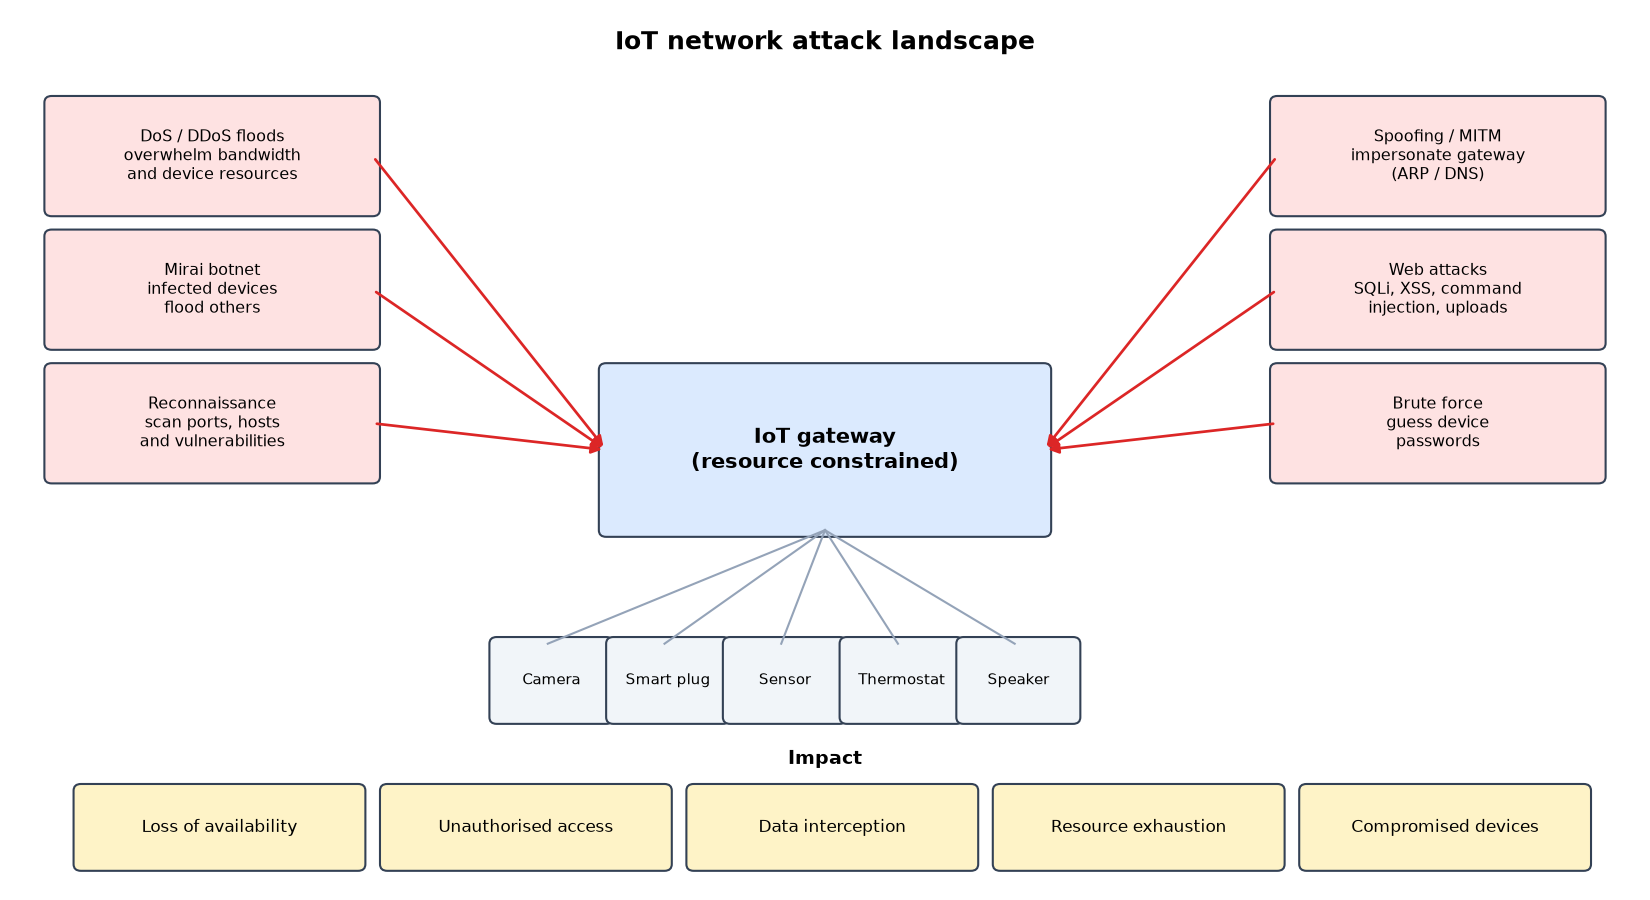
\includegraphics[width=\linewidth]{iot_attack_landscape.png}
    \caption{IoT network attack landscape and potential impact of cyberattacks.}
    \label{fig:iot_attack_landscape}
\end{figure}

To address this requirement, Intrusion Detection Systems (IDS) are used to monitor network traffic and identify suspicious or malicious activities. An IDS analyses the traffic or the features associated with the incoming traffic\cite{abdulganiyu2023systematic}, helps identify normal versus malicious behaviour, and raises an alert when suspicious activity is detected. Traditional IDS approaches may rely on predefined signatures or rules, which can limit their ability to recognise changing attack patterns\cite{khraisat2019survey}. Therefore, ML and DL-based approaches have been explored, because they can learn patterns from network traffic without relying only on predefined attack signatures\cite{rakine2025comprehensive}. ML-based IDS approaches can perform binary classification, where network traffic is classified as either normal or malicious. However, binary classification does not provide information about the specific type of attack\cite{palshikar2022distinguishes}, and different types of attacks need to be mitigated with different responses. A multiclass IDS can further classify malicious traffic into specific attack categories, providing more detailed information about the nature of the detected attack. However, although ML/DL-based multiclass IDS can provide detailed attack classification, their computational and memory requirements can make deployment challenging in resource-constrained IoT environments\cite{mallidi2025advancements}.

Due to the limited resources and memory of IoT devices, running a complex ML/DL-based model can be a problem. Therefore, lightweight and resource-efficient IDS models are required for resource-constrained IoT environments\cite{arshad2020intrusion}. For this, resource optimisation techniques can be used to reduce the resource requirements of ML/DL models, and one of these approaches is quantization\cite{gholami2022survey}. Quantization reduces the numerical precision used to represent the parameters of a model, which reduces the model size and computational requirements while maintaining detection performance. Therefore, quantizing the IDS can make the multiclass detection system more suitable for resource-constrained IoT environments\cite{misrak2025lightweight}.

But resource efficiency alone cannot address the challenge of detecting previously unseen or zero-day attacks\cite{el2024advanced}. Existing IDS and ML/DL-based models are trained using known traffic and attack patterns, and when traffic behaves differently from the patterns seen during training\cite{sabeel2021building}, classification of attacks can be difficult. Therefore, detecting abnormal behaviour is important in addition to classifying known attack types. Anomaly detection can identify traffic behaviour that differs from normal behaviour, which makes it useful for detecting potentially unseen attack patterns. One traffic characteristic that can be used for identifying unseen attacks is the packet Inter-Arrival Time (IAT), which is the interval of time between two consecutive packets\cite{sahin2025leveraging}.

\begin{figure}[htbp]
    \centering
    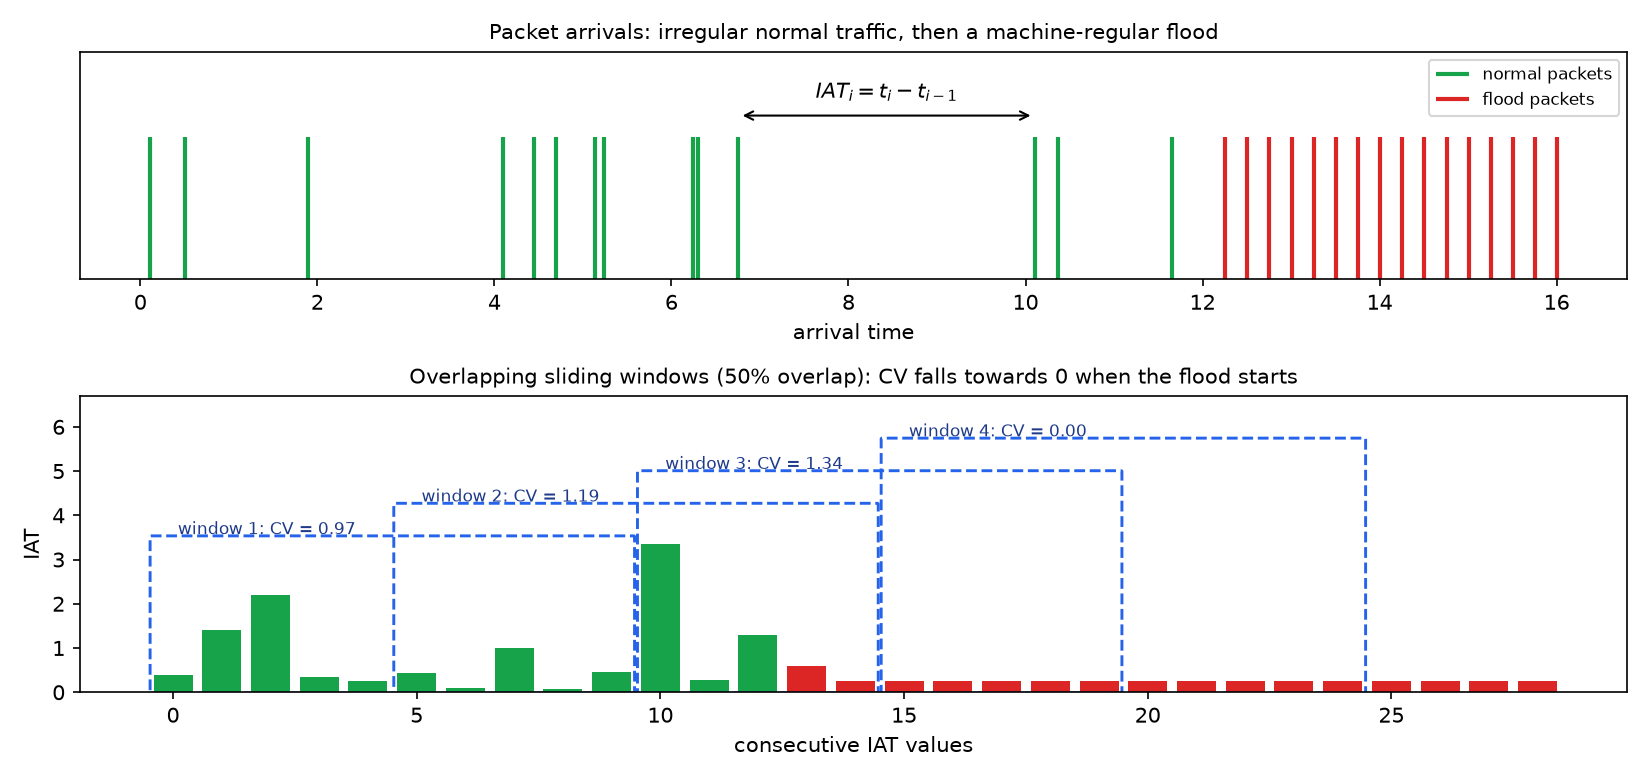
\includegraphics[width=\linewidth]{iat_diagram.png}
    \caption{Illustration of Packet Inter-Arrival Time (IAT) and sliding windows over consecutive IAT values.}
    \label{fig:iat}
\end{figure}

To analyse the variations in packet inter-arrival time, a sliding-window approach can be used to check the traffic behaviour over the incoming packets. In each window, the IAT values of the incoming consecutive packets are considered and their standard deviation is calculated to measure the variation in packet arrival time and frequency. If the behaviour of the window is found to be abnormal, the traffic is considered potentially anomalous, and this anomaly can trigger the multiclass IDS for further classification of the suspicious traffic\cite{toupas2019intrusion}. The multiclass IDS can classify the suspicious traffic into the corresponding attack category based on the traffic patterns, and based on the identified type an appropriate mitigation technique can be applied to the incoming suspicious traffic; for example, rate limiting and traffic filtering are used to mitigate DDoS attacks. After applying the specific mitigation technique, the network can be analysed again to determine whether the abnormal behaviour of the traffic has been reduced, and if the abnormal behaviour is still present, further mitigation can be initiated.

Based on the above challenges, there is a need for an IoT intrusion detection system that can address resource constraints, detect abnormal attack behaviour and also support appropriate mitigation\cite{heidari2023internet}. Therefore, this work proposes a resource-constrained multiclass intrusion detection and mitigation system for IoT networks and devices. The proposed approach uses the packet inter-arrival time with sliding-window analysis to identify abnormal traffic behaviour. A quantized multiclass IDS is then used to classify the suspicious traffic into different categories of attack, and based on the identified type of attack an appropriate mitigation technique is applied\cite{mondal2026quantized}, followed by re-analysis of the network traffic to verify the reduction of the anomaly. The overall approach aims to provide a lightweight and resource-efficient mechanism for detecting, classifying and mitigating malicious activities in resource-constrained IoT networks.

\subsection{Novelty}
The novelty of our work is that, instead of running a heavy multiclass IDS on every traffic window, our system first uses a lightweight IAT-based fuzzy logic module, and only the suspicious or attack windows are forwarded to the classifier and then to the mitigation module. The same timing features that the first module has already measured are reused by the third module to contain unseen attacks, and the first module is run again after every mitigation action to check that it worked. The main contributions of this work are:

\begin{enumerate}
\item A three-stage IDS (detect, classify, mitigate) in which 54.9\% of the windows of an end-to-end stream bypassed the multiclass module, so the classifier does not have to run on every traffic window.
\item A fuzzy logic module that combines the coefficient of variation, packet rate and IAT deviation of a window with a behaviour deviation score learned only from normal traffic. On the same 1,360 test windows it achieved 99.81\% F1-score and 99.77\% recall, whereas the static CV threshold and adaptive median--MAD methods reached only 4.39\% and 1.44\% recall, and the IAT timing features alone reached 15.91\%.
\item A measured accuracy-versus-memory trade-off for the classifier stage, where the Random Forest gives 90.85\% accuracy (94.56\% at window level) at 6.29 ms per window, while the INT8 post-training quantized neural network needs only 16.2 KB, which is 74.6\% smaller than its FP32 version, and runs in 0.55 ms per window with 77.85\% accuracy.
\item An evaluation on three held-out Mirai categories, where the fuzzy logic module detected 100\% of the unseen attack windows and a nearest-neighbour open-set check labelled 100\% of them as unknown, while the confidence-based rejection of our earlier classifier detected 0\% of them.
\item An attack-specific mitigation module that maps the 31 known CICIoT2023 classes into 10 attack policy families and picks the containment of unseen attacks from their traffic shape. Each action is verified by re-running the first module, and across all 33 attack classes 95.7\% of the mitigations brought the traffic back to the normal risk zone.
\end{enumerate}


% =====================================================================================
\section{Literature Survey}
% =====================================================================================
Several proposed IDS systems use packet features like MAC address, packet length, source IP and destination IP\cite{ppdowdaorsuttf2026}. However, these attributes contain sensitive and private information, leading to privacy concerns. To address this problem, a paper demonstrated how IAT can detect stealthy slow DoS and spoofing attacks on IoT networks. Recent studies have used IAT with deep learning and reinforcement learning models, but these attacks were tested in simulated lab environments, which questions their real-life effectiveness. Although several papers implemented similar IDS, most focus on attack detection, while effective attack mitigation remains comparatively limited. Therefore, this research aims to preserve privacy and explore appropriate mitigation mechanisms for IoT systems.

Existing multiclass intrusion detection techniques often segment network traffic into temporal sliding windows to observe how normal traffic morphs into malicious activity\cite{whffi2026}. Conventional frameworks evaluate deep convolutional feature extractors against handcrafted summary statistics, finding that simpler statistical descriptors with tree-based classifiers like XGBoost can outperform complex deep learning models. However, calculating over a hundred statistical attributes per block introduces processing latency, making such pipelines impractical for resource-constrained IoT devices. Furthermore, these supervised models remain vulnerable to novel zero-day attacks and lack automated mitigation mechanisms to suppress detected threats.

Similarly, other prevailing intrusion detection strategies focus on identifying compromised hardware nodes using statistical outlier rejection and time-frequency spectral transforms\cite{wtai2025}. These architectures extract temporal traffic statistics across sliding windows, compress them using deep autoencoders, and employ swarm-optimised classifiers to identify anomalies. Despite reasonable detection accuracy, these multi-stage processes incur significant computational and memory overheads. Moreover, detection accuracy and responsiveness degrade under elevated attack intensities, and the framework ultimately stops at flagging infected nodes without providing autonomous countermeasures.

Current papers have proposed an edge-friendly intrusion detection approach for resource-constrained IoT environments using Boosted Convolutional Trees (BCT)\cite{eict2025}. Existing CNN/LSTM-based IDS algorithms can provide effective intrusion detection, but their model size and computational requirements are very large, which makes deployment challenging. BCT combines 1D convolutional feature extraction, soft decision trees and boosting, and was evaluated using CIC-IoT2023, X-IIoTID and Edge-IIoTset. BCT achieved competitive intrusion-detection performance with a smaller model size and faster inference than CNN/LSTM approaches. However, its performance can be affected by imbalanced attack classes, and the model was not fully deployed, tested and validated in physical real-world environments.

Another paper proposed a lightweight intrusion detection system for IoT environments using improved feature engineering and advanced dynamic quantization\cite{lidsfiot2025}. It used a combination of RAL-MIFS, two-stage IPCA, DNN-BiLSTM, QAT, PTDQ and Optuna for feature selection, dimensionality reduction, intrusion classification and hyperparameter optimisation, with QAT and PTDQ integrated to reduce the resource consumption of the model. The data used for evaluation were CIC-IDS2017 and CIC-IoT2023. The paper reported high detection and classification performance with a considerable reduction in model size after quantization. However, class imbalance remains a challenge, especially for minority attack classes, and the evaluation was not done on actual resource-constrained IoT devices.

Another paper proposed a lightweight dynamic threshold method for real-time network anomaly detection on edge devices\cite{dynamic_ids2025}. It combines a 30-second sliding window, the 3$\sigma$ statistical rule, a Kolmogorov--Smirnov normality check and protocol-aware filtering, tracking just two features: packets per second and bytes per second. Tested on CICIDS2017, NSL-KDD and simulated industrial traffic, it achieved 94.7\%--96.2\% accuracy with only 5.1\% CPU usage and fewer false alarms. However, it assumes fairly normal traffic behaviour, struggles with non-stationary patterns like periodic spikes, and has not been validated on a real industrial system in the long term.

Another paper presented an energy-conscious deep learning framework for intrusion detection built specifically for edge computing devices\cite{energy_ids2025}. It combines SeparableConv1D layers, SMOTE, structured pruning and quantization-aware training to keep feature extraction lightweight, deal with class imbalance and shrink the model size. Tested on NSL-KDD and deployed on a Raspberry Pi 4, it achieved 86.2\% accuracy using just 94,408 parameters, with 3.6$\times$ faster inference and 60\% less power draw compared with LSTM-based models. However, the model still misses a good number of attack instances even after tuning the threshold, and since it is only tested on NSL-KDD, it is not clear how well it would hold up on real, mixed IoT traffic.

In summary, the existing works usually optimise only one of detection accuracy, resource efficiency or zero-day robustness, and most of them stop at detection without applying and verifying a mitigation. Our system combines a label-free timing-based anomaly filter, a quantized multiclass classifier that runs only when needed, an open-set check for unseen attacks, and an attack-specific mitigation module that verifies its own actions.


% =====================================================================================
\section{Proposed Methodology}
% =====================================================================================
The proposed resource-constrained multiclass intrusion detection system detects anomalous network traffic by analysing the inter-arrival time (IAT) and the behaviour of the incoming traffic, then identifies the type of attack happening in the IoT network, and finally applies and verifies the mitigation according to that type. To achieve this, the proposed system contains three modules: an IAT-based fuzzy anomaly detection module (Module 1), a multiclass attack identification module (Module 2) and an attack-specific mitigation module (Module 3). The key objective of the first module is to determine whether the incoming network traffic shows anomalous behaviour, using the timing, rate and behaviour of the traffic in a sliding window and a Mamdani fuzzy inference system. If the traffic is normal, it continues without further processing and the second and third modules stay idle. When suspicious or attack behaviour is detected, the window is forwarded to the second module to identify the corresponding attack type, or to recognise that it is unknown. The third module then takes the action for the identified attack, and after applying the action the traffic is checked again with the first module to verify that the attack risk has come back to normal. The overall workflow of our system is shown in Fig.~\ref{fig:workflow}, and the following subsections discuss the modules in detail.

\begin{figure}[htbp]
\centering
\resizebox{\textwidth}{!}{%
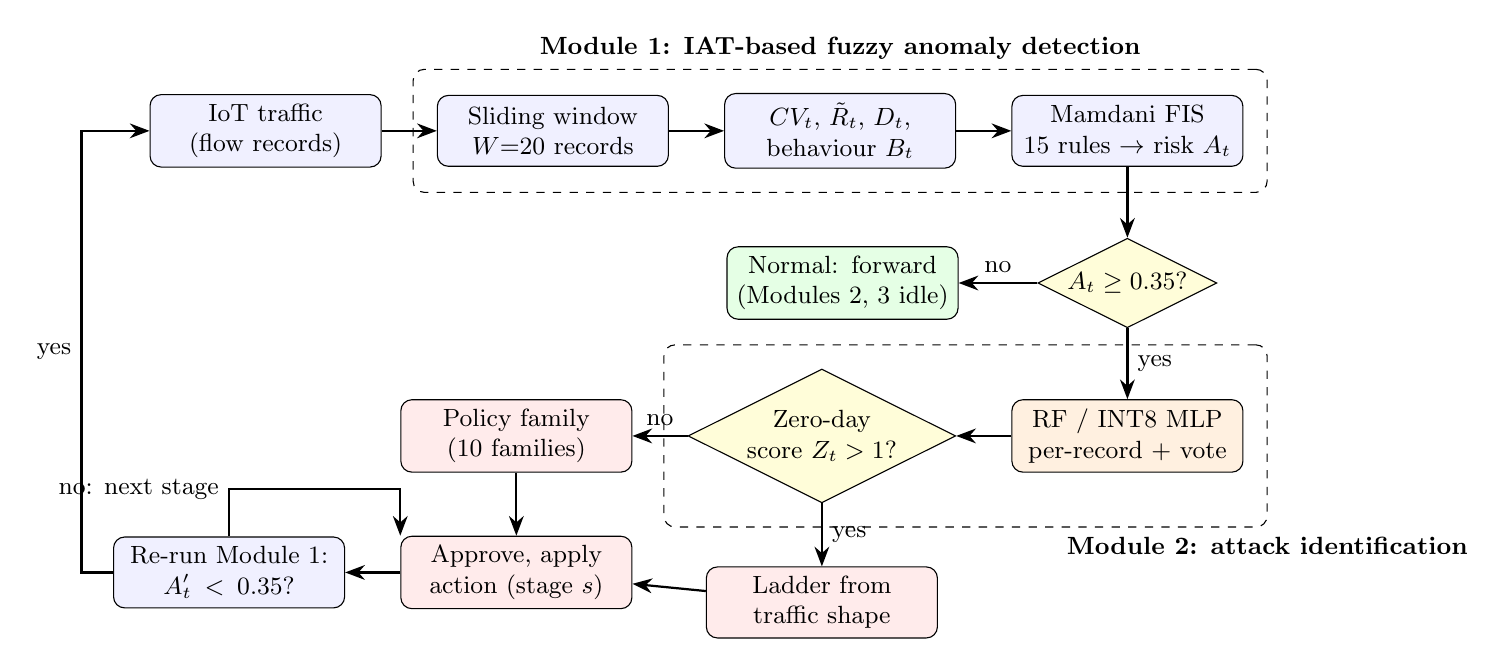
\begin{tikzpicture}[
  node distance=5mm and 7mm,
  box/.style={draw, rounded corners, align=center, minimum height=9mm, text width=27mm, font=\small, fill=blue!6},
  m2/.style={box, fill=orange!12},
  m3/.style={box, fill=red!8},
  ok/.style={box, fill=green!10},
  dec/.style={draw, diamond, aspect=2, align=center, font=\small, inner sep=1pt, fill=yellow!15},
  arr/.style={-{Stealth[length=2.5mm]}, thick}]
\node[box] (in) {IoT traffic\\(flow records)};
\node[box, right=of in] (win) {Sliding window\\$W{=}20$ records};
\node[box, right=of win] (feat) {$CV_t$, $\tilde{R}_t$, $D_t$,\\behaviour $B_t$};
\node[box, right=of feat] (fis) {Mamdani FIS\\15 rules $\rightarrow$ risk $A_t$};
\node[dec, below=9mm of fis] (gate) {$A_t \ge 0.35$?};
\node[ok, left=10mm of gate] (pass) {Normal: forward\\(Modules 2, 3 idle)};
\node[m2, below=9mm of gate] (clf) {RF / INT8 MLP\\per-record + vote};
\node[dec, left=of clf] (zd) {Zero-day\\score $Z_t>1$?};
\node[m3, below=8mm of zd] (shape) {Ladder from\\traffic shape};
\node[m3, left=of zd] (pol) {Policy family\\(10 families)};
\node[m3, below=8mm of pol] (act) {Approve, apply\\action (stage $s$)};
\node[box, left=of act] (ver) {Re-run Module 1:\\$A'_t<0.35$?};
\begin{scope}[on background layer]
\node[draw, dashed, rounded corners, fit=(win)(feat)(fis), inner sep=3mm, label={[font=\small\bfseries]above:Module 1: IAT-based fuzzy anomaly detection}] {};
\node[draw, dashed, rounded corners, fit=(clf)(zd), inner sep=3mm, label={[font=\small\bfseries]below right:Module 2: attack identification}] {};
\end{scope}
\draw[arr] (in) -- (win);
\draw[arr] (win) -- (feat);
\draw[arr] (feat) -- (fis);
\draw[arr] (fis) -- (gate);
\draw[arr] (gate) -- node[above,font=\small]{no} (pass);
\draw[arr] (gate) -- node[right,font=\small]{yes} (clf);
\draw[arr] (clf) -- (zd);
\draw[arr] (zd) -- node[above,font=\small]{no} (pol);
\draw[arr] (zd) -- node[right,font=\small]{yes} (shape);
\draw[arr] (pol) -- (act);
\draw[arr] (shape) -- (act);
\draw[arr] (act) -- (ver);
\draw[arr] (ver.north) -- ++(0,6mm) node[left,font=\small]{no: next stage} -| (act.north west);
\draw[arr] (ver.west) -- ++(-4mm,0) |- node[near start,left,font=\small]{yes} (in.west);
\end{tikzpicture}}
\caption{Overall workflow of the proposed system. Module 1 checks every window, only suspicious or attack windows are sent to Module 2, and Module 3 applies the attack-specific or shape-based action and verifies it with Module 1.}
\label{fig:workflow}
\end{figure}


\subsection{Dataset Preparation}
The CICIoT2023 dataset is captured from 105 real IoT devices and is given as flow-level records with 46 numeric features and 34 labels: benign traffic and 33 attacks grouped into 7 families (DDoS, DoS, Mirai, Reconnaissance, Spoofing, Web-based and Brute Force). Because the training file is 1.6~GB, it is read in chunks and sampled with a cap per class, which gives 153,135 training records. The separate test file gives 37,187 test records, which are never used for training or calibration. To evaluate unseen attacks, all three Mirai classes (Mirai-greeth\_flood, Mirai-greip\_flood and Mirai-udpplain) are excluded from the training of Module 2 and from every threshold and policy, and are only used at test time.


% -------------------------------------------------------------------------------------
\subsection{IAT-Based Fuzzy Anomaly Detection Module (Module 1)}
% -------------------------------------------------------------------------------------
The IAT-based fuzzy anomaly detection module determines whether the incoming IoT network traffic exhibits anomalous behaviour. It uses the packet inter-arrival time, sliding windows, statistical feature extraction, a normal traffic baseline and fuzzy logic to give the attack risk of every window. Normal traffic continues along the normal path, whereas suspicious or attack traffic is forwarded to the multiclass attack identification module.

\subsubsection{Input Records and Inter-Arrival Time}
The CICIoT2023 dataset is given in the form of flow-level records, and it does not have the raw packet timestamps. Each record already contains the inter-arrival time ($\mathrm{IAT}_i$) calculated by the feature extractor of the dataset, as well as the packet rate ($\mathrm{Rate}_i$), the number of packets and the flow duration. We do not create any artificial timestamps; the given $\mathrm{IAT}_i$ is directly used as the timing signal of the traffic. Since the rows of the public CSV files are shuffled, the evaluation windows are assembled from the test records of the traffic class under test, optionally mixed with benign background records (Section~\ref{sec:setup}).

\subsubsection{Sliding Windows}
The records are divided into sliding windows of $W = 20$ records. In a live deployment consecutive windows overlap by 50\% (step $S = 10$), so the older window and the latest window share some records, and window $t$ covers the records $[tS,\; tS + W - 1]$. For evaluation, the ground-truth label of each window is given by the fraction of attack records present in it:
\begin{equation}
  a_t = \frac{1}{W}\sum_{i=1}^{W} \mathbf{1}\!\left(y_i \neq \text{Benign}\right),
  \qquad
  y_t =
  \begin{cases}
    1, & a_t \ge 0.5\\
    0, & \text{otherwise}
  \end{cases}
\end{equation}
Here, $y_i$ represents the label of the $i$-th record in the window, $a_t$ represents the fraction of attack records in window $t$, and $y_t$ denotes the label of the window, which is 1 if half or more of the records are attack records and 0 otherwise.

\subsubsection{Window Feature Extraction}
From the IAT and rate values of each window, statistical features are calculated to understand the traffic behaviour. First, the mean IAT ($\mu_t$) is calculated as follows:
\begin{equation}
  \mu_t = \frac{1}{W}\sum_{i=1}^{W}\mathrm{IAT}_i
\end{equation}
Here, $W$ represents the number of records in a window, and $\mu_t$ represents the average IAT of that window. Using this, the standard deviation ($\sigma_t$) is calculated as follows:
\begin{equation}
  \sigma_t = \sqrt{\frac{1}{W}\sum_{i=1}^{W}\left(\mathrm{IAT}_i-\mu_t\right)^2}
\end{equation}
Here, $\sigma_t$ represents the standard deviation of the IAT values and indicates the variation of the arrival intervals around their mean. To measure the relative variation in the IAT values, the coefficient of variation (CV) is determined as follows:
\begin{equation}
  CV_t = \frac{\sigma_t}{\mu_t + \epsilon}, \qquad \epsilon = 10^{-12}
\end{equation}
Here, $CV_t$ represents the coefficient of variation of the current window. A higher CV indicates greater relative variation in the arrival intervals, whereas a lower CV indicates more consistent intervals. Next, to measure the volume of traffic, the packet rate of the window ($\tilde{R}_t$) is calculated as the median of the record rates:
\begin{equation}
  \tilde{R}_t = \operatorname{Median}\left(\mathrm{Rate}_1, \ldots, \mathrm{Rate}_W\right)
\end{equation}
The median is used instead of the mean because the rate feature of CICIoT2023 is heavy-tailed, and a single benign record with an extreme rate would otherwise raise the mean of the whole window and cause a false alarm. Then the IAT deviation ($D_t$) is calculated to check how much the mean IAT of the current window differs from the mean IAT of normal traffic:
\begin{equation}
  D_t = \frac{\left|\mu_t-\mu_{N}\right|}{\mu_{N}}
\end{equation}
Here, $\mu_N$ represents the mean IAT of normal traffic, which is obtained from the normal traffic baseline (Section~\ref{sec:baseline}).

Normal IoT traffic shows natural random variation in the arrival of packets, and its CV stays around 1 (the median CV of benign training windows is 1.00). In flooding attacks like DoS/DDoS, the attack tools send packets at almost constant intervals, due to which the CV goes close to 0; in our data the median window CV is 0.001 for DDoS and below 0.001 for DoS. In slow scanning attacks the probes are irregular and widely spaced, which increases both the CV and $D_t$. Since attacks can make the CV go either \emph{down} or \emph{up}, using only an upper threshold on the CV is not enough, because it will miss the flooding attacks. Therefore we use fuzzy logic with multiple inputs to take the decision.

Timing features alone are also not enough when the attack does not change the timing of the traffic. Reconnaissance, spoofing, web and brute-force records have a window CV close to that of benign traffic, and when normal background records are mixed into a flood window, they break its regular timing. Therefore, a fourth input, the behaviour deviation ($B_t$), is calculated. All 46 record features are compressed with $x \mapsto \operatorname{sign}(x)\log(1+|x|)$ and standardised with the mean and standard deviation of benign training records. For each record $i$ in the window, $d_i$ is the mean Euclidean distance to its $k=5$ nearest benign training records, and the behaviour deviation is:
\begin{equation}
  B_t = \frac{\operatorname{Median}\left(d_1, \ldots, d_W\right)}{\theta_B}
\end{equation}
Here, $\theta_B$ is the 99th percentile of the same statistic over 1,000 windows of held-out benign training records, so $B_t > 1$ means that the window is more unusual than 99\% of normal windows. $B_t$ is learned only from normal traffic and does not use any attack label, so Module 1 remains an unsupervised anomaly detector and can still detect unseen attacks.

\subsubsection{Normal Traffic Baseline}\label{sec:baseline}
The normal traffic baseline is calculated only from benign training traffic; no attack traffic, and in particular no held-out attack traffic, is used for it. The baseline stores the mean normal IAT ($\mu_N$), the median and percentiles of the normal window CV values, the median normal rate, and the benign reference records and threshold $\theta_B$ used for $B_t$. The median and the median absolute deviation (MAD) of normal CV values are calculated as follows:
\begin{equation}
  M = \operatorname{Median}(CV), \qquad
  \mathrm{MAD} = \operatorname{Median}\left(\left|CV - M\right|\right)
\end{equation}
Here, $M$ represents the median of the normal CV values, and $\mathrm{MAD}$ represents the median absolute deviation of the normal CV values from their median. The median of the normal CV ($M = 1.00$) is used as the centre of the Medium CV membership function, and $\mu_N$ is used to calculate $D_t$.

\subsubsection{Mamdani Fuzzy Inference}
A Mamdani fuzzy inference system takes the four window features $(CV_t, \tilde{R}_t, D_t, B_t)$ as input and gives a continuous attack risk $A_t \in [0,1]$ as output. Each input has three linguistic terms (Low, Medium, High), defined using triangular (\texttt{trimf}) and trapezoidal (\texttt{trapmf}) membership functions, which are given in Table~\ref{tab:mf}. These terms are based on the behaviour of normal traffic: the normal CV stays around its median ($M \approx 1.0$), normal windows have a very small IAT deviation, and the Low/Medium boundary of $B_t$ lies just above the 99th percentile of normal windows.

\begin{table}[htbp]
\tbl{Membership functions of the fuzzy inputs and output.}
{\begin{tabular}{llll}
\toprule
Variable & Low & Medium & High \\
\midrule
$CV_t$ $[0,6]$             & trimf(0, 0, 0.65)   & trimf(0.50, $M$, 1.55)   & trapmf(1.40, 1.80, 6, 6) \\
$\tilde{R}_t$ $[0,50000]$  & trimf(0, 0, 350)    & trimf(200, 600, 1500)    & trapmf(1000, 2500, 50000, 50000) \\
$D_t$ $[0,5]$              & trimf(0, 0, 0.18)   & trimf(0.12, 0.35, 0.65)  & trapmf(0.50, 0.90, 5, 5) \\
$B_t$ $[0,10]$             & trimf(0, 0, 1.15)   & trimf(1.0, 1.3, 1.7)     & trapmf(1.4, 1.9, 10, 10) \\
$A_t$ $[0,1]$              & trimf(0, 0, 0.35)   & trimf(0.25, 0.50, 0.75)  & trapmf(0.60, 0.85, 1, 1) \\
\bottomrule
\end{tabular}}
\label{tab:mf}
\end{table}

\begin{figure}[htbp]
\centering
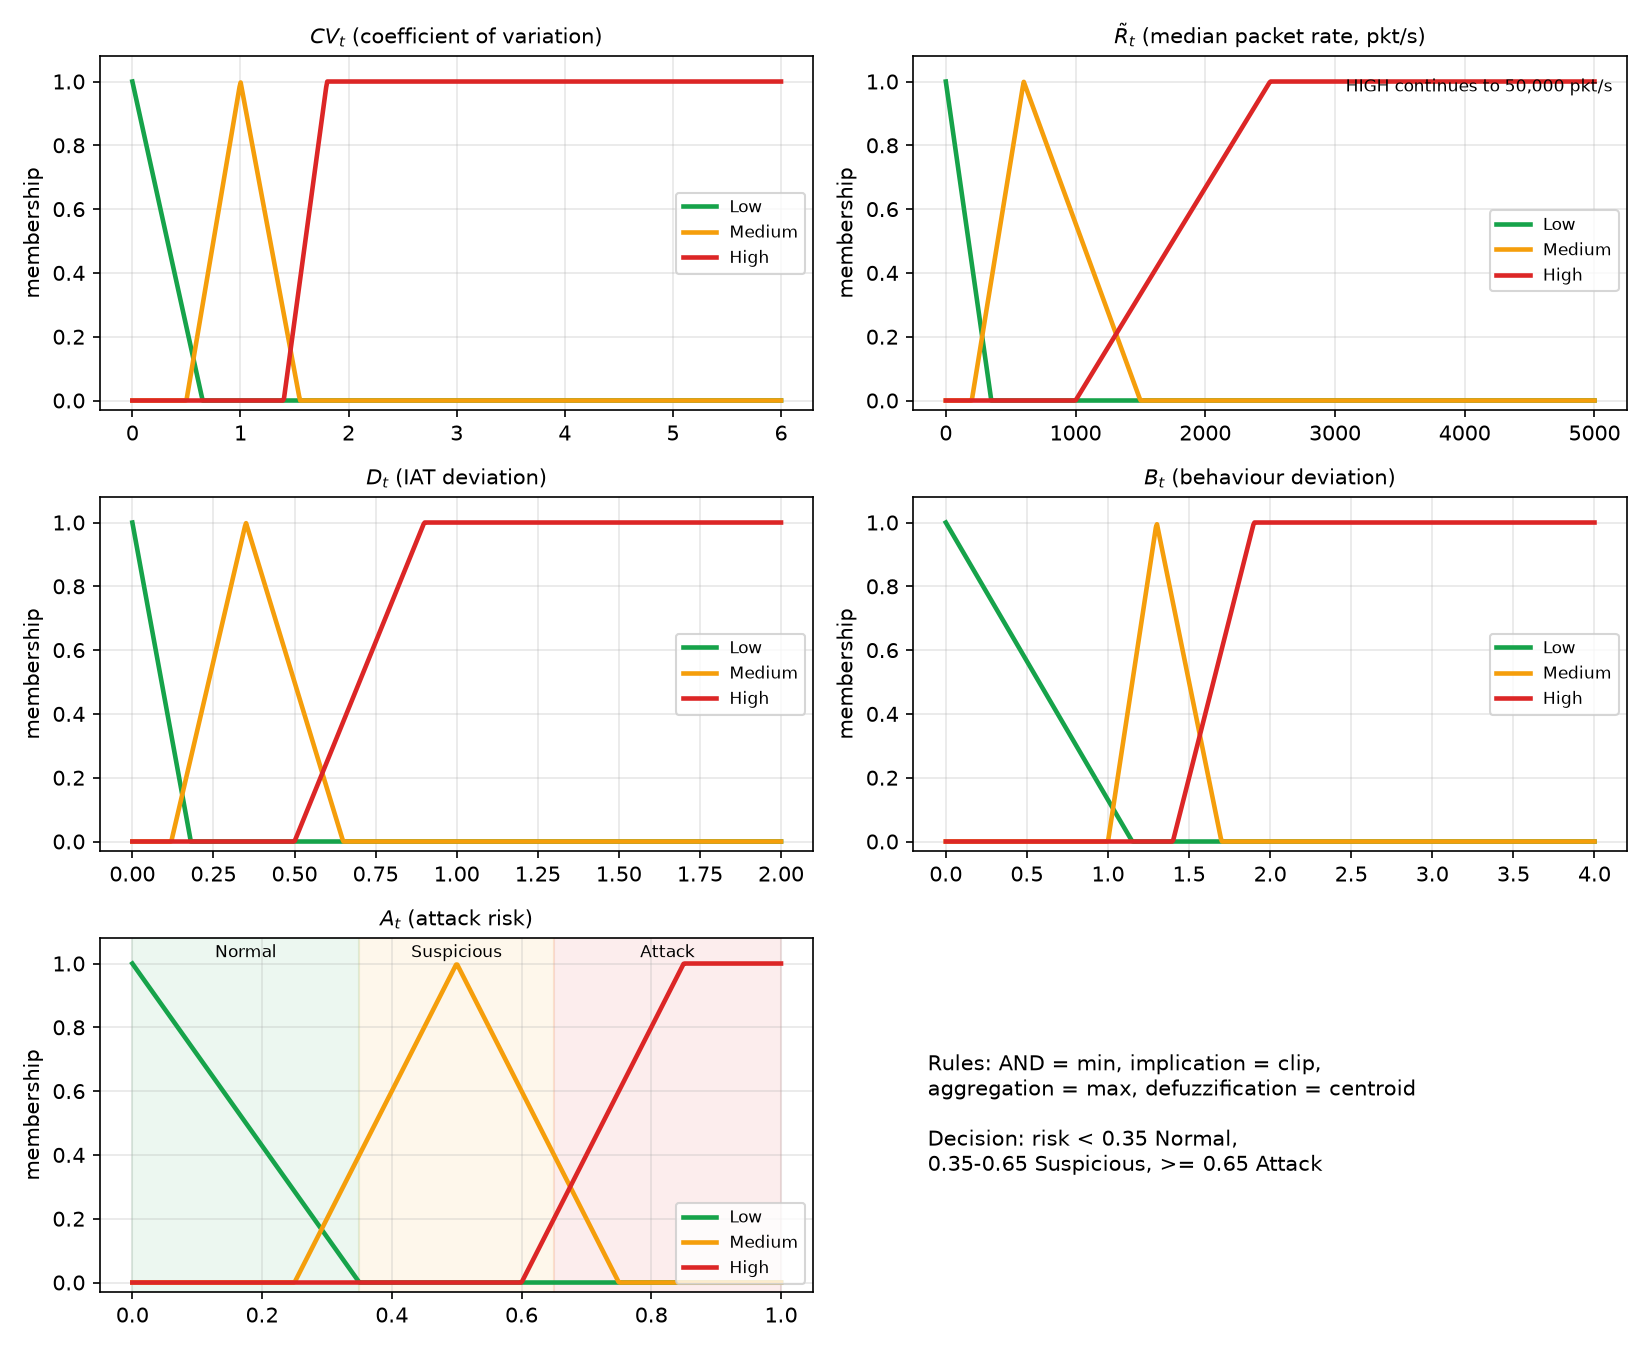
\includegraphics[width=\textwidth]{fig_membership_functions.png}
\caption{Membership functions of the fuzzy inputs $CV_t$, $\tilde{R}_t$, $D_t$, $B_t$ and the output attack risk $A_t$ with Normal, Suspicious and Attack zones.}
\label{fig:mf}
\end{figure}

The fuzzy inference system consists of 15 Mamdani fuzzy rules, given in Table~\ref{tab:rules}. Rules 4--13 detect timing and volume anomalies; for example, rule 12 captures constant-rate floods with an abnormally low CV and a high rate. Rules 1--3 describe normal traffic and also require the behaviour to be normal, and rules 14 and 15 raise the risk when the records do not resemble normal traffic. The strength of a rule is the minimum of the membership degrees of its IF part (AND = min), each rule clips its output set at that strength, and the clipped sets are combined with the maximum operator. The final attack risk is obtained by centroid defuzzification:
\begin{equation}
  A_t = \frac{\int z\,\mu_{\mathrm{agg}}(z)\,dz}{\int \mu_{\mathrm{agg}}(z)\,dz}
\end{equation}
Here, $z$ represents the values of the attack risk, $\mu_{\mathrm{agg}}(z)$ represents the combined output membership of all the rules, and $A_t$ denotes the final attack risk of window $t$. To measure the benefit of $B_t$, a timing-only variant with the three inputs $(CV_t, \tilde{R}_t, D_t)$ and the 13 original rules (rules 1--13 without the $B_t$ conditions) is also evaluated.

\begin{table}[htbp]
\tbl{Fuzzy rule base.}
{\begin{tabular}{cll}
\toprule
\# & IF & THEN Risk \\
\midrule
1  & $CV_t$ Medium $\wedge$ $\tilde{R}_t$ Low $\wedge$ $D_t$ Low $\wedge$ $B_t$ Low & Low \\
2  & $CV_t$ Low $\wedge$ $\tilde{R}_t$ Low $\wedge$ $D_t$ Low $\wedge$ $B_t$ Low & Low \\
3  & $CV_t$ Medium $\wedge$ $\tilde{R}_t$ Low $\wedge$ $D_t$ Medium $\wedge$ $B_t$ Low & Low \\
4  & $CV_t$ High $\wedge$ $\tilde{R}_t$ High & High \\
5  & $CV_t$ High $\wedge$ $D_t$ High & High \\
6  & $\tilde{R}_t$ High $\wedge$ $D_t$ High & High \\
7  & $CV_t$ Medium $\wedge$ $\tilde{R}_t$ High & High \\
8  & $CV_t$ High $\wedge$ $\tilde{R}_t$ Medium & High \\
9  & $CV_t$ Medium $\wedge$ $\tilde{R}_t$ Medium $\wedge$ $D_t$ Medium & Medium \\
10 & $\tilde{R}_t$ High & High \\
11 & $D_t$ High & High \\
12 & $CV_t$ Low $\wedge$ $\tilde{R}_t$ High & High \\
13 & $CV_t$ High $\wedge$ $\tilde{R}_t$ Low & Medium \\
14 & $B_t$ High & High \\
15 & $B_t$ Medium & Medium \\
\bottomrule
\end{tabular}}
\label{tab:rules}
\end{table}

\subsubsection{Decision and Hand-off to Module 2}
The attack risk obtained from the fuzzy logic controller is used to classify the incoming traffic into three categories:
\begin{equation}
  \text{Decision}_t =
  \begin{cases}
    \text{Normal},     & A_t < 0.35\\
    \text{Suspicious}, & 0.35 \le A_t < 0.65\\
    \text{Attack},     & A_t \ge 0.65
  \end{cases}
\end{equation}
If the traffic is identified as normal, it continues without further processing and the second module stays idle, which saves the computation and power of the IoT device. If the traffic is identified as suspicious or attack, the window is considered anomalous ($\hat{y}_t = 1$) and is forwarded to the multiclass attack identification module to determine the type of attack.

\subsubsection{Statistical Baselines for Comparison}
To compare the performance of the fuzzy logic, two simple statistical methods are also implemented on the same windows. In the first method, the \emph{static CV threshold}, the window is considered anomalous if $CV_t > P_{95}$, where $P_{95}$ is the 95th percentile of normal CV values. In the second method, the \emph{adaptive median--MAD threshold}, a history $H_t$ of CV values from previously accepted normal windows (maximum 500 values) is maintained, and the adaptive threshold ($T_t$) is calculated as follows:
\begin{equation}
  T_t = \operatorname{Median}(H_t) + k\cdot \operatorname{MAD}(H_t), \qquad k = 3
\end{equation}
Here, $T_t$ represents the adaptive threshold, and $k$ is a sensitivity parameter that controls the threshold level. If $CV_t > T_t$, the window is flagged as anomalous. To make sure that attack traffic does not get added to the normal history, $CV_t$ is added to $H_t$ only when $CV_t \le T_t$ and the fuzzy risk $A_t < 0.35$.


% -------------------------------------------------------------------------------------
\subsection{Multiclass Attack Identification Module (Module 2)}
% -------------------------------------------------------------------------------------
Once the IAT-based fuzzy anomaly detection module identifies that the incoming traffic window is anomalous, the flagged window is forwarded to the multiclass attack identification module. The main objective of this second module is to classify what type of attack is happening in the network, or to recognise that it is an unseen zero-day attack, while keeping the computation small for resource-constrained IoT devices. To perform this operation, the module uses a record-level classifier with window voting, an INT8 post-training quantized neural network for edge devices, and a nearest-neighbour open-set check for unknown attacks.

\begin{figure}[htbp]
\centering
\resizebox{\textwidth}{!}{%
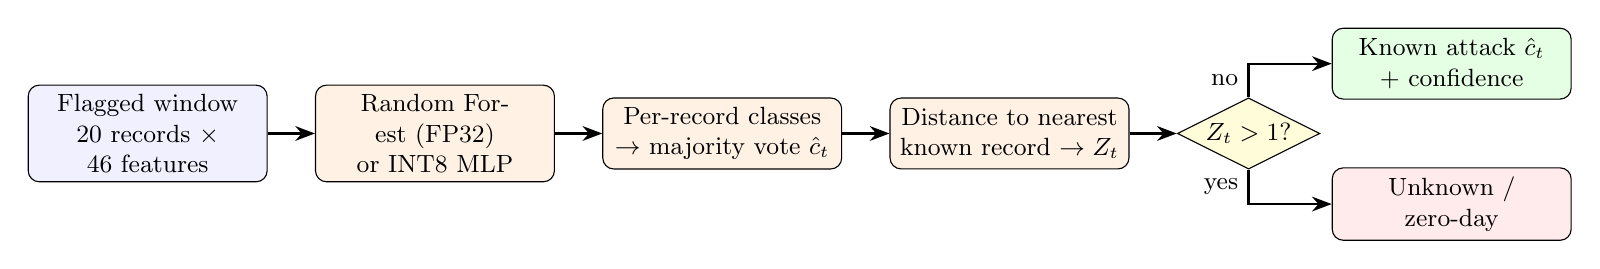
\begin{tikzpicture}[
  node distance=5mm and 6mm,
  box/.style={draw, rounded corners, align=center, minimum height=9mm, text width=28mm, font=\small, fill=orange!10},
  dec/.style={draw, diamond, aspect=2, align=center, font=\small, inner sep=1pt, fill=yellow!15},
  arr/.style={-{Stealth[length=2.5mm]}, thick}]
\node[box, fill=blue!6] (w) {Flagged window\\20 records $\times$ 46 features};
\node[box, right=of w] (rf) {Random Forest (FP32)\\or INT8 MLP};
\node[box, right=of rf] (vote) {Per-record classes\\$\rightarrow$ majority vote $\hat{c}_t$};
\node[box, right=of vote] (nn) {Distance to nearest\\known record $\rightarrow Z_t$};
\node[dec, right=of nn] (d) {$Z_t > 1$?};
\node[box, above right=2mm and 6mm of d, fill=green!10] (k) {Known attack $\hat{c}_t$\\+ confidence};
\node[box, below right=2mm and 6mm of d, fill=red!8] (u) {Unknown /\\zero-day};
\draw[arr] (w) -- (rf); \draw[arr] (rf) -- (vote); \draw[arr] (vote) -- (nn); \draw[arr] (nn) -- (d);
\draw[arr] (d) |- node[near start,left,font=\small]{no} (k);
\draw[arr] (d) |- node[near start,left,font=\small]{yes} (u);
\end{tikzpicture}}
\caption{Workflow of the multiclass attack identification module: record-level classification, window voting and the open-set zero-day check.}
\label{fig:module2}
\end{figure}

\subsubsection{Features}
The second module uses all 46 numeric flow features of the CICIoT2023 dataset, including the timing and rate features (IAT, Rate, Srate, Drate, flow\_duration, Duration), the size features (Header\_Length, Tot~sum, Tot~size, Min, Max, AVG, Std, Number, Magnitude, Radius, Covariance, Variance, Weight), the TCP flag numbers and counts, and the protocol indicators (HTTP, HTTPS, DNS, Telnet, SMTP, SSH, IRC, TCP, UDP, DHCP, ARP, ICMP, IPv, LLC). The labels are never used as input. The classifier is trained on 31 known classes, which are benign traffic and 30 known attack classes. The three Mirai classes are excluded from training and validation and are reserved for the unseen-attack evaluation, and 15\% of the known training records are held out as a validation set for calibration.

\subsubsection{Random Forest with Window Voting}
The main classifier is a Random Forest with 60 trees, a maximum depth of 20, at least 3 samples per leaf and balanced class weights per bootstrap sample. Each of the $W = 20$ records of a flagged window is classified, and the window label is decided by a majority vote over the records predicted as attacks:
\begin{equation}
  \hat{c}_t =
  \begin{cases}
    \arg\max_{c \neq \text{Benign}} \; n_t(c), & \sum_{c \neq \text{Benign}} n_t(c) \ge 0.3\,W\\
    \text{Benign}, & \text{otherwise}
  \end{cases}
\end{equation}
Here, $n_t(c)$ represents the number of records in window $t$ predicted as class $c$. The benign background records are ignored when the attack records make up at least 30\% of the window. The confidence of the decision is the mean predicted probability of $\hat{c}_t$ over the voting records. If the second module finds only benign traffic, it overrules the alarm of the first module and no mitigation is applied.

\subsubsection{INT8 Post-Training Quantization}
Storing and processing a 32-bit floating-point (FP32) model takes more memory and processing power, which is not ideal for resource-constrained IoT devices. For edge deployment, a multilayer perceptron with the structure 46 $\rightarrow$ 128 $\rightarrow$ 64 $\rightarrow$ 31 (ReLU activations, softmax output) is trained using the Adam optimiser (learning rate $2\times10^{-3}$, batch size 512, early stopping on 10\% of the training data). Its inputs are log-compressed and quantized to 8-bit integers with a per-feature affine quantizer fitted on the training minimum and maximum:
\begin{equation}
  s = \frac{r_{\max}-r_{\min}}{255}, \qquad
  z = \operatorname{round}\!\left(-128 - \frac{r_{\min}}{s}\right), \qquad
  q = \operatorname{clip}\!\left(\operatorname{round}\!\left(\tfrac{r}{s}\right) + z,\,-128,\,127\right)
\end{equation}
Here, $s$ represents the scale factor, $z$ represents the zero-point offset, and $q$ is the quantized 8-bit integer value, which is clipped to stay within $[-128, 127]$; the real value is recovered as $r \approx s\,(q - z)$. After training, the input standardisation is folded into the first layer, the weights of each layer are quantized symmetrically to INT8 ($w_q = \operatorname{round}(w / s_w)$, $s_w = \max|w| / 127$), and the activations are quantized to INT8 with scales calibrated on 5,000 training records (99.9th percentile). The matrix products are computed as INT8 $\times$ INT8 $\rightarrow$ INT32 accumulations and rescaled afterwards, as on a microcontroller or a DSP.

\subsubsection{Unknown-Attack Detection}
A supervised classifier always predicts one of the known classes, so if a new or unseen attack enters the network, it will be wrongly classified as one of the known attacks. In our earlier experiments, the rejection of predictions with a low maximum softmax probability detected none of the unseen Mirai traffic, because the classifier was more confident on the unseen floods than on the known traffic. Therefore, we use an open-set check based on the distance in feature space. The training records of the known classes (a random subset of 60,000) are log-compressed, standardised and stored in a nearest-neighbour index, and for a flagged window the zero-day score is:
\begin{equation}
  Z_t = \frac{\operatorname{Median}_{i \in \mathcal{A}_t}\; \min_{j} \left\lVert \mathbf{x}_i - \mathbf{x}_j^{\text{train}} \right\rVert}{\theta_Z}
\end{equation}
Here, $\mathcal{A}_t$ represents the set of records predicted as attacks in window $t$, $\mathbf{x}_j^{\text{train}}$ represents the stored known training records, and $\theta_Z$ is the 97.5th percentile of the same statistic over windows of the validation set. The final decision of the second module is:
\begin{equation}
  \hat{Y}_t =
  \begin{cases}
    \hat{c}_t, & Z_t \le 1\\
    \text{Unknown / zero-day}, & Z_t > 1
  \end{cases}
\end{equation}
If $Z_t > 1$, the window is anomalous but further from every known class than 97.5\% of the known validation windows, so it is flagged as a possible zero-day attack instead of being forced into a known class. The output of this module is the predicted attack class, its confidence, the zero-day flag, and the mask of records predicted as attacks, which is used by the third module.


% -------------------------------------------------------------------------------------
\subsection{Attack-Specific Mitigation Module (Module 3)}
% -------------------------------------------------------------------------------------
After the multiclass attack identification module identifies the type of attack, or reports that it is unknown, the result is passed to the mitigation module, which takes the action according to the identified type. The main objective of this third module is to apply the correct response for each attack family, to contain the attack when it is a zero-day attack for which no policy is available, and to check that the response has actually worked. To perform this operation, the module uses an external policy file that maps every known attack class to a policy family and its escalation ladder, a shape-based containment that is used when no policy matches, an approval rule, and a graduated escalation loop that keeps checking the traffic with the first module until the attack risk comes back to normal.

\subsubsection{Attack-Specific Mitigation Policies}
The mitigation policies are kept in an external JSON file instead of hardcoded conditions, so that new attack classes can be added without changing the code. All 31 known classes of the CICIoT2023 dataset are mapped into 10 attack policy families (plus benign), and each family has its own escalation ladder, which starts with the least disruptive action (Table~\ref{tab:playbooks}). The families follow how an attack is stopped rather than how it is named; for example, SYN, PSH-ACK and RST-FIN floods share the TCP state exhaustion policy, because all of them are stopped by stateful filtering and SYN cookies, while UDP and ICMP floods share the volumetric flood policy. Every action also has an action class that tells how the action changes the traffic: FILTER means that the traffic of the source is limited or filtered, BLOCK means that the traffic of that source is stopped or isolated, and ALERT means that nothing is changed and only the operator is informed. Each policy additionally gives long-term recommendations and a class-specific tip, for example a shorter header timeout for SlowLoris or parameterised queries for SQL injection.

\begin{table}[htbp]
\tbl{Mapping of CICIoT2023 classes to policy families and their escalation ladders (assumed efficacy of each action in brackets).}
{\small
\begin{tabular}{lll}
\toprule
Policy family (classes) & Escalation ladder & Auto threshold \\
\midrule
Volumetric flood (UDP, ICMP, TCP, SynonymousIP floods) & rate limit (0.75) $\rightarrow$ block (0.98) $\rightarrow$ blackhole (0.97) & 0.60 \\
TCP state exhaustion (SYN, PSH-ACK, RST-FIN floods) & SYN cookies (0.80) $\rightarrow$ rate limit $\rightarrow$ block & 0.60 \\
Fragmentation (ICMP, UDP, ACK fragmentation) & drop fragments (0.80) $\rightarrow$ rate limit $\rightarrow$ block & 0.60 \\
Slow application (SlowLoris, HTTP floods) & limit connections (0.80) $\rightarrow$ block & 0.60 \\
Reconnaissance (scans, sweeps, vulnerability scan) & block scanner (0.97) $\rightarrow$ isolate segment (0.97) & 0.60 \\
Spoofing / MITM (ARP, DNS spoofing) & ARP/DNS integrity (0.95) $\rightarrow$ isolate segment & 0.65 \\
Web application (SQLi, XSS, command injection, ...) & WAF rule (0.85) $\rightarrow$ block & 0.70 \\
Credential (dictionary brute force) & throttle logins (0.85) $\rightarrow$ block & 0.70 \\
Malware / backdoor & quarantine endpoint (0.97) & admin \\
Botnet (no class after holding out Mirai) & rate limit $\rightarrow$ isolate device (0.95) & 0.70 \\
Zero-day (by traffic shape) & see Table~\ref{tab:shape} & -- \\
\bottomrule
\end{tabular}}
\label{tab:playbooks}
\end{table}

The actions are selected according to the behaviour of each attack. For example, flooding attacks are rate limited instead of isolating the device, because these attacks mostly come from spoofed sources, so isolating a local device will not stop the attack and it may also cut off an innocent device. Similarly, scanning attacks can't be rate limited because they already use a very low rate, so the source is blocked. For web application attacks a WAF rule is applied instead of blocking the source, because blocking can also stop the legitimate users. The three Mirai classes are not added to the Botnet policy, because they are held out from training as the zero-day attack, and if they matched a policy the held-out experiment would no longer be valid.

\subsubsection{Shape-Based Containment for Zero-Day Attacks}
When a zero-day attack enters the network, the classifier can't give its name, so no policy will match, and only raising an alert would not stop the attack. To handle this, our system uses the shape of the traffic, measured on the records that the second module marked as attack, with the same features that the first module uses. The coefficient of variation, mean packet rate and IAT deviation are enough to understand the shape of the attack even without knowing its name, and the containment is selected as given in Table~\ref{tab:shape}:
\begin{equation}
  \text{Shape}_t =
  \begin{cases}
    \text{Constant-rate flood}, & CV_t < 0.05 \;\text{or}\; \left(CV_t < 0.65 \wedge \bar{R}_t > R_{50}\right)\\
    \text{Volumetric surge}, & \bar{R}_t > R_{95} \wedge D_t > 0.5\\
    \text{Slow probe}, & CV_t > 1.40 \wedge \bar{R}_t \le R_{95}\\
    \text{Volumetric surge}, & \bar{R}_t > R_{95}\\
    \text{Unclassified anomaly}, & \text{otherwise}
  \end{cases}
  \label{eq:shape}
\end{equation}
Here, $\bar{R}_t$ represents the mean rate of the suspicious records, and $R_{50}$ and $R_{95}$ represent the median and 95th percentile of the mean rate of benign windows. The breakpoints of $CV_t$ and $D_t$ are the same as in the membership functions of the first module, so the shape classes match the rules that flagged the window. The condition $CV_t < 0.05$ is used because no benign window in CICIoT2023 has a CV below about 0.23, so such regular timing is machine-generated whatever the packet rate; some Mirai GRE floods have a per-record rate below the benign median, which the rate condition alone would miss. The shape is measured on the suspicious records only, because the benign background records of the same window would hide, for example, the regular timing of a flood.

\begin{table}[htbp]
\tbl{Shape-based containment selected for zero-day windows (Eq.~\ref{eq:shape}).}
{\begin{tabular}{lll}
\toprule
Observed behaviour & Identified shape & Containment ladder \\
\midrule
$CV_t$ near 0, or low with rate above normal median & Constant-rate flood & rate limit $\rightarrow$ block $\rightarrow$ blackhole \\
$\bar{R}_t$ above normal $P_{95}$, $D_t$ high & Volumetric surge & rate limit $\rightarrow$ blackhole $\rightarrow$ isolate \\
$CV_t$ high, $\bar{R}_t$ not high & Slow probe / scan & block source $\rightarrow$ isolate segment \\
Flagged but no known shape & Unclassified anomaly & rate limit $\rightarrow$ block $\rightarrow$ isolate \\
\bottomrule
\end{tabular}}
\label{tab:shape}
\end{table}

\subsubsection{Automatic Execution or Analyst Approval}
The first action of a known attack is executed automatically only if four conditions hold: the confidence of the second module reaches the threshold of the policy (0.60--0.75), the policy does not require an administrator, the attack is known, and the action only filters or limits the traffic. Actions that block or isolate traffic always need an analyst, because a wrong decision would cut off legitimate devices. For a zero-day window, a reversible rate limit may start automatically, but any blocking stage waits for an analyst. In this way, the system gives fast automatic responses for confident flood decisions and prevents blocking traffic on uncertain or unknown decisions.

\subsubsection{Graduated Escalation and Verification}
After selecting the ladder, the mitigation is applied in a graduated manner, which means the least disruptive action is applied first and the stronger action is applied only if the traffic does not become normal. The action is applied through a network controller, which is simulated in this work. It filters the records that the second module predicted as attacks, and each targeted record is removed with a probability equal to the assumed efficacy $e$ of the action. The ground-truth labels are not used, so classification errors carry through to the mitigation result. The removed records are replaced by benign records, since legitimate traffic keeps arriving. The share of the attack traffic volume removed by an action is calculated as follows:
\begin{equation}
  S_t = \left(1 - \frac{\sum_{i \in \mathcal{A}'_t} \mathrm{Rate}_i}{\sum_{i \in \mathcal{A}_t} \mathrm{Rate}_i}\right) \times 100
\end{equation}
Here, $\mathcal{A}_t$ represents the targeted records of the window before the action, $\mathcal{A}'_t$ represents the targeted records that still get through after the action, and $S_t$ denotes the percentage of the targeted packet volume removed by that action. After applying the action, the first module, with all four inputs, is run again on the window after mitigation, and the new attack risk is calculated as follows:
\begin{equation}
  A'_t = f_{\mathrm{FIS}}\left(CV'_t,\ \tilde{R}'_t,\ D'_t,\ B'_t\right)
\end{equation}
Here, $A'_t$ represents the attack risk of the window after mitigation, and the primed features are measured again on that window, so the change of the packet timing is measured rather than assumed. The attack is considered contained when this risk comes back into the normal range:
\begin{equation}
  \text{Decision}_t =
  \begin{cases}
    \text{Contained}, & A'_t < 0.35\\
    \text{Escalate to the next action}, & A'_t \ge 0.35
  \end{cases}
\end{equation}
If the risk is still above the threshold, the next action of the ladder is applied, for example rate limiting is escalated to blocking the source and then to isolating the segment. If the risk stays high after all stages, the incident is escalated to the security team. It should be noted that in the current work the actions are not applied on a real network; they are applied on the recorded traffic, and the efficacy of each action is an assumption of the simulation. However, the verification uses the same detector and features as the first module, so a window counts as contained only if its timing and behaviour look normal again.


% =====================================================================================
\section{Result Analysis}
% =====================================================================================
This section checks the performance of the proposed IoT intrusion detection system on the CICIoT2023 dataset. The results are analysed in terms of detection accuracy, precision, recall, F1-score and false-positive rate for the first module; classification accuracy, macro-F1, inference latency and model size for the second module; held-out attack detection; and mitigation performance and end-to-end behaviour for the third module.

\subsection{Experimental Setup}\label{sec:setup}
The proposed system is implemented in Python with scikit-learn, NumPy and pandas, all random seeds are fixed, and a Streamlit dashboard shows every step of the pipeline. The anomaly detection module uses sliding windows of 20 records, and a Mamdani fuzzy logic controller assigns an attack risk from 0 to 1, where a score below 0.35 shows normal traffic, a score from 0.35 to 0.65 indicates suspicious traffic, and a score of 0.65 or above indicates an attack. The following evaluations are used:
\begin{itemize}
\item \textbf{Module 1}: 1,360 windows of 20 test records, 40 for each of the 34 classes (40 normal windows, 1,200 windows of the 30 known attacks and 120 windows of the 3 held-out Mirai classes). All four detectors (static CV, adaptive MAD, timing-only fuzzy and final fuzzy) are run on the same windows in a shuffled order.
\item \textbf{Module 2}: record level on all 32,687 test records of the 31 known classes, and window level on windows of 70\% attack records and 30\% benign background records (30 windows per attack class).
\item \textbf{Module 3}: 645 windows driven by the predictions of the second module, 15 windows for each of the 33 attack classes (80\% attack and 20\% benign records) and 150 normal windows.
\item \textbf{End to end}: a stream of normal, DDoS-SYN, Recon-PortScan, Mirai-udpplain and DoS-UDP phases (39 windows per run, each attack window containing 80\% attack records), repeated with 10 random seeds, giving 390 windows.
\end{itemize}
Latency is measured on a desktop CPU.

\subsection{Anomaly Detection Performance}
The anomaly detection module is tested by comparing the static CV threshold, the adaptive MAD threshold, the timing-only fuzzy logic and the final fuzzy logic with the behaviour deviation, on the same 1,360 windows (Table~\ref{tab:anomaly_performance} and Fig.~\ref{fig:anomaly_comparison}). The static CV and adaptive MAD methods detected only 4.39\% and 1.44\% of the attack windows, because both of them only test for an unusually \emph{high} CV, while flooding attacks lower it. The timing-only fuzzy logic detected 15.91\% of the attack windows with a precision of 99.06\%: it is very precise but misses most attacks, because a flood window that contains a few benign records loses its regular timing, and attacks such as reconnaissance or web exploits do not change the timing at all. With the behaviour deviation $B_t$, the fuzzy logic achieved an accuracy of 99.63\%, a precision of 99.85\%, a recall of 99.77\%, an F1-score of 99.81\% and a balanced accuracy of 97.39\%. All four methods have the same false-positive rate of 5.0\% (2 of 40 normal windows), and the false alarms of the fuzzy logic are checked again by the second module instead of being blocked. Since only 40 normal windows are used here, each normal window changes the false-positive rate by 2.5 percentage points.

\begin{table}[htbp]
\tbl{Performance comparison of anomaly detection methods on the same 1,360 test windows.}
{\begin{tabular}{lcccccc}
\toprule
\textbf{Method} & \textbf{Accuracy} & \textbf{Precision} & \textbf{Recall} & \textbf{F1-Score} & \textbf{Bal. Acc.} & \textbf{FPR} \\
\midrule
Static CV threshold          & 7.06\%  & 96.67\% & 4.39\%  & 8.41\%  & 49.70\% & 5.00\% \\
Adaptive MAD ($k=3$)         & 4.19\%  & 90.48\% & 1.44\%  & 2.83\%  & 48.22\% & 5.00\% \\
Fuzzy logic (timing only)    & 18.24\% & 99.06\% & 15.91\% & 27.42\% & 55.45\% & 5.00\% \\
Fuzzy logic (timing + $B_t$) & 99.63\% & 99.85\% & 99.77\% & 99.81\% & 97.39\% & 5.00\% \\
\bottomrule
\end{tabular}}
\label{tab:anomaly_performance}
\end{table}

\begin{figure}[htbp]
\centering
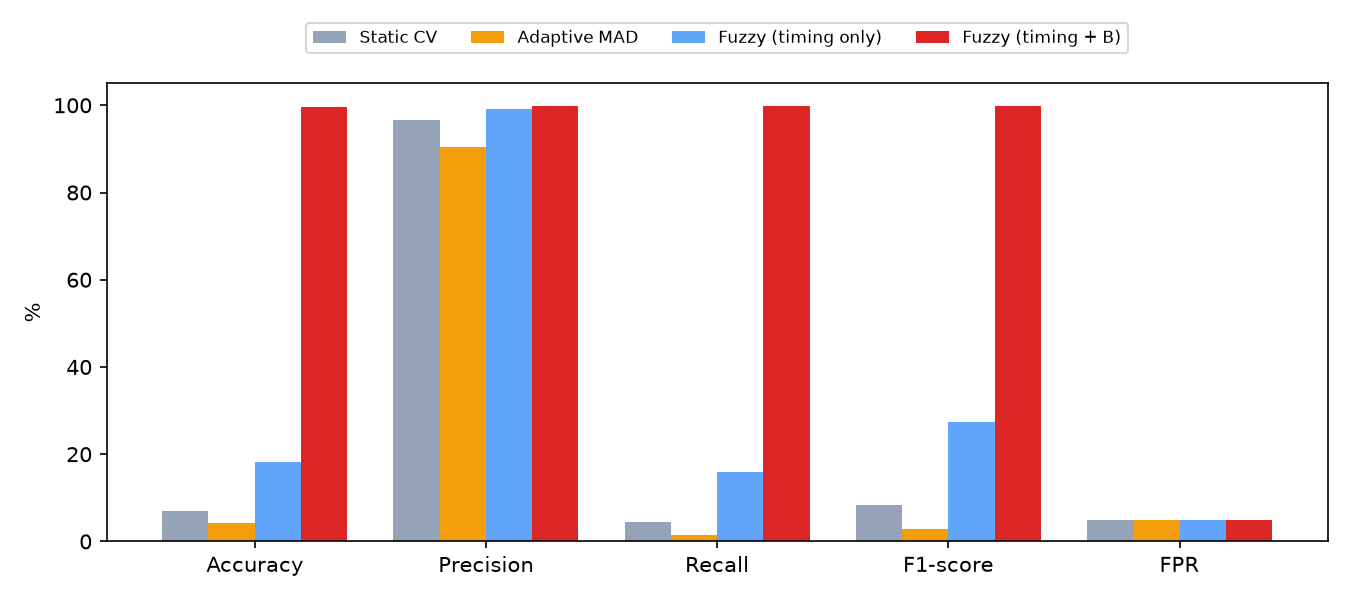
\includegraphics[width=\textwidth]{fig_anomaly_detection_comparison.png}
\caption{Comparison of the static CV, adaptive MAD, timing-only fuzzy and final fuzzy methods on accuracy, precision, recall, F1-score and false-positive rate over the same 1,360 test windows.}
\label{fig:anomaly_comparison}
\end{figure}

The confusion matrices of the four methods are given in Fig.~\ref{fig:anomaly_cm}: the threshold methods and the timing-only fuzzy logic place most attack windows in the normal class, whereas the final fuzzy logic recovers 1,317 of the 1,320 attack windows. The behaviour of the methods on the normal, known attack and held-out cohorts is shown in Fig.~\ref{fig:cohorts}, and the share of windows flagged for each traffic family is shown in Fig.~\ref{fig:m1family}. Every attack family is detected in at least 98.5\% of its windows, and the lowest class is Recon-OSScan. The first module needs about 2.7~ms per window on a desktop CPU.

\begin{figure}[htbp]
\centering
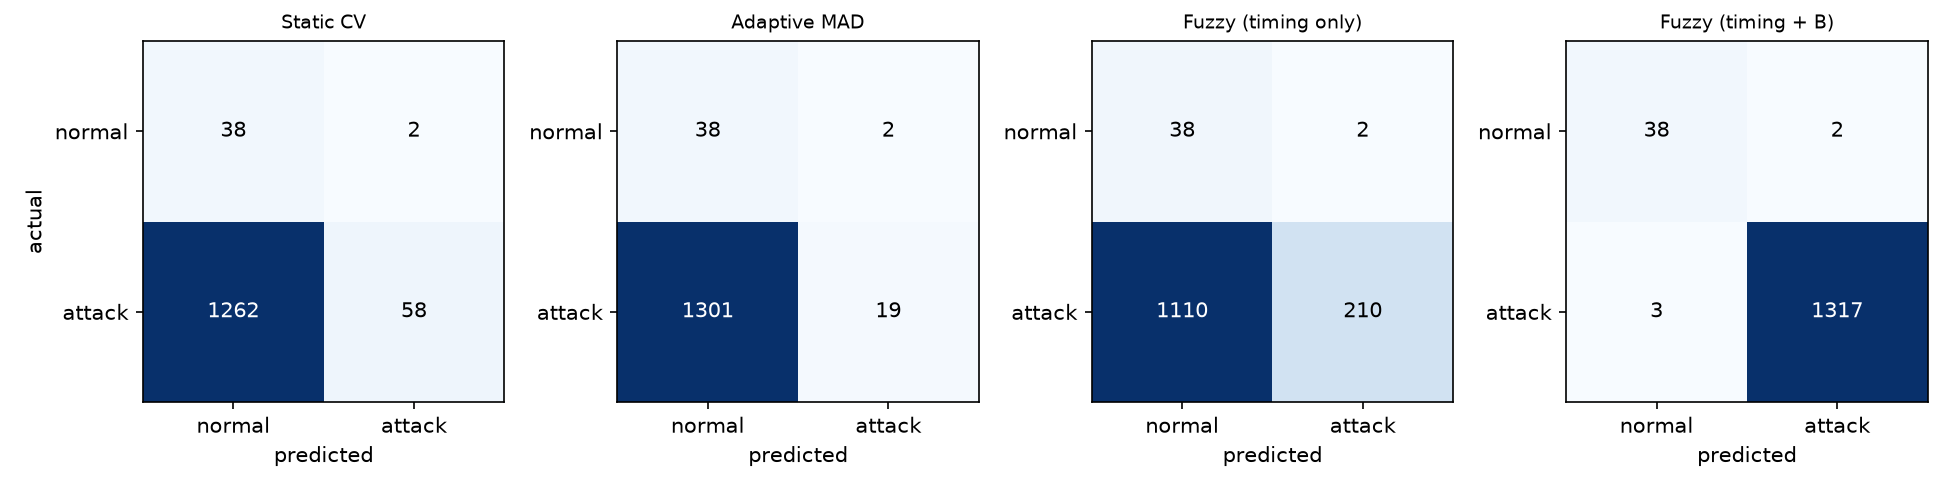
\includegraphics[width=\textwidth]{fig_anomaly_confusion_matrices.png}
\caption{Confusion matrices of the four anomaly detection methods on 1,360 windows (40 normal, 1,320 attack).}
\label{fig:anomaly_cm}
\end{figure}

\begin{figure}[htbp]
\centering
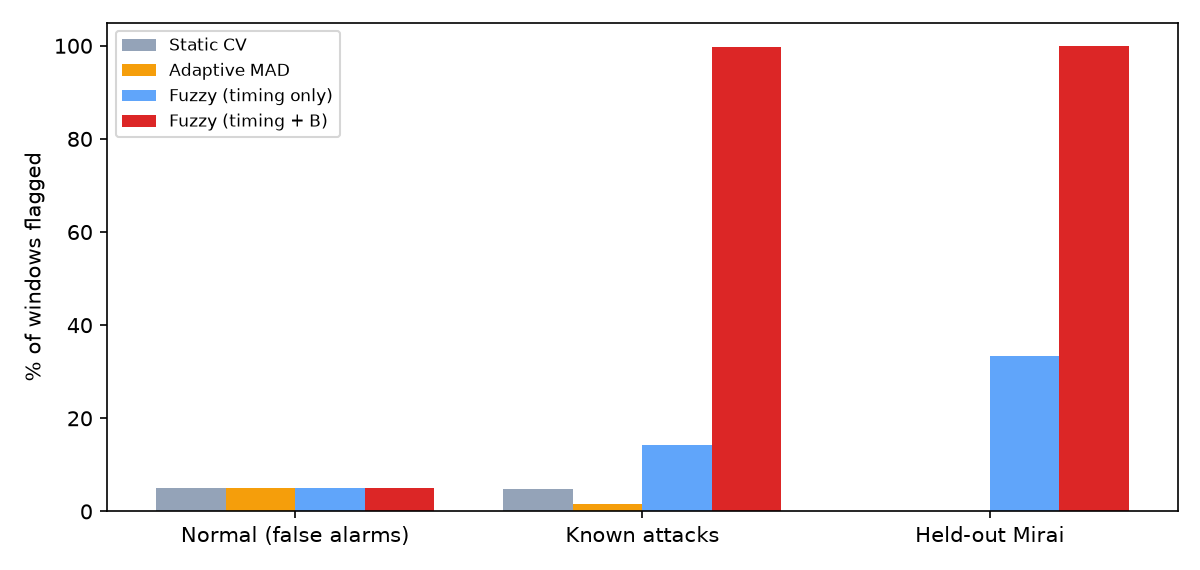
\includegraphics[width=0.85\textwidth]{fig_cohort_detection_rates.png}
\caption{Windows flagged by each method on the normal, known attack and held-out Mirai cohorts. For the normal cohort the bars are false alarms, and for the other two cohorts they are detections.}
\label{fig:cohorts}
\end{figure}

\begin{figure}[htbp]
\centering
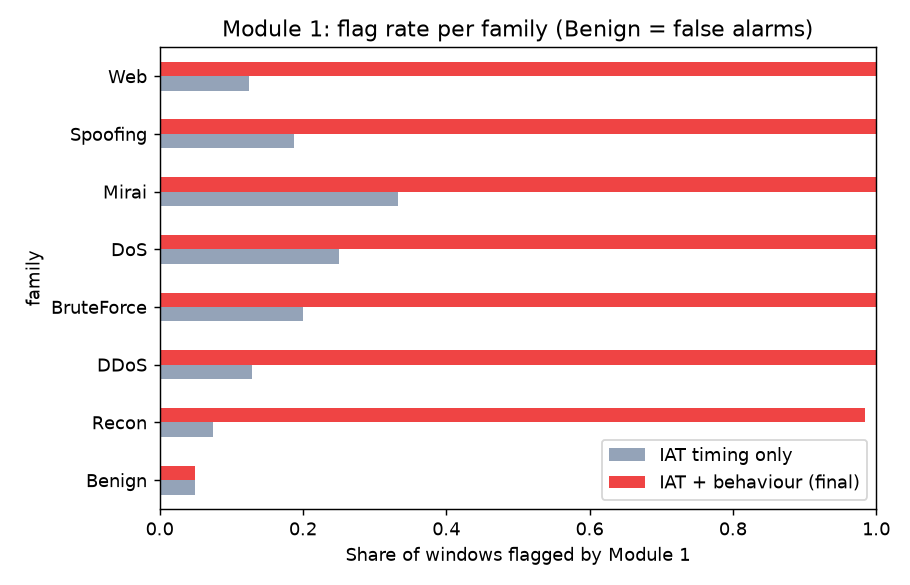
\includegraphics[width=0.8\textwidth]{m1_flag_rate_by_family.png}
\caption{Share of windows flagged by Module 1 for each traffic family, with and without the behaviour deviation input (for the Benign family this is the false-alarm rate).}
\label{fig:m1family}
\end{figure}

\subsection{Multiclass Classification Performance}
Table~\ref{tab:classification_performance} shows the record-level performance of the second module on the 31 known classes. The Random Forest achieved an accuracy of 90.85\%, a macro-F1 score of 79.34\% and a weighted-F1 score of 91.22\%. Its accuracy at attack-family level, which decides the mitigation policy, is 93.42\%. At window level, with 30\% benign background records, the voting rule raised the accuracy to 94.56\% for the exact class and 95.44\% for the family. All flood classes (DDoS and DoS) reached an F1-score of at least 0.97 (Fig.~\ref{fig:m2perclass}). The weaker classes are the rare web and reconnaissance attacks, which have very few records in the dataset, such as SQL injection (0.37), XSS (0.46), uploading attack (0.32) and Recon-PingSweep (0.29), and their errors mostly stay inside the correct family (Fig.~\ref{fig:m2family}). The FP32 multilayer perceptron achieved 77.95\% accuracy and 83.57\% family accuracy, and after INT8 quantization it achieved 77.85\% and 83.49\%, a drop of only 0.1 percentage points, with 98.51\% prediction agreement with the FP32 model. The comparison of the three classifiers is also shown in Fig.~\ref{fig:multiclass}.

\begin{table}[htbp]
\tbl{Performance comparison of the multiclass classification models (record level, 32,687 test records of 31 known classes; latency per window of 20 records).}
{\begin{tabular}{lccccc}
\toprule
\textbf{Model} & \textbf{Accuracy} & \textbf{Macro-F1} & \textbf{Family Acc.} & \textbf{Latency (ms)} & \textbf{Size} \\
\midrule
Random Forest (FP32) & 90.85\% & 79.34\% & 93.42\% & 6.29 & 118.3 MB \\
MLP (FP32)           & 77.95\% & 63.15\% & 83.57\% & --   & 63.6 KB \\
MLP (INT8)           & 77.85\% & 63.17\% & 83.49\% & 0.55 & 16.2 KB \\
\bottomrule
\end{tabular}}
\label{tab:classification_performance}
\end{table}

\begin{figure}[htbp]
\centering
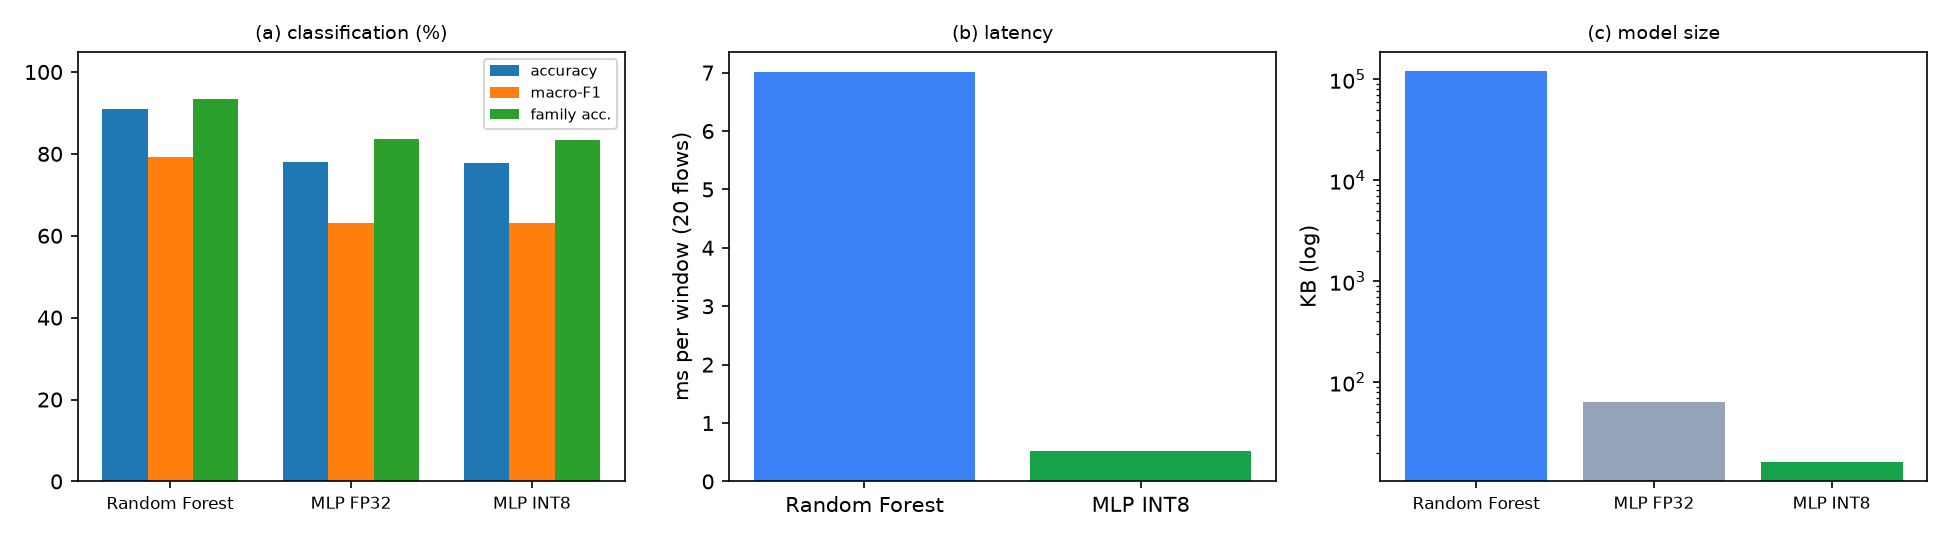
\includegraphics[width=\textwidth]{fig_multiclass_comparison.png}
\caption{Comparison of the Random Forest, FP32 MLP and INT8 MLP on (a) classification performance, (b) inference latency per window of 20 records, and (c) model size on a log scale.}
\label{fig:multiclass}
\end{figure}

\begin{figure}[htbp]
\centering
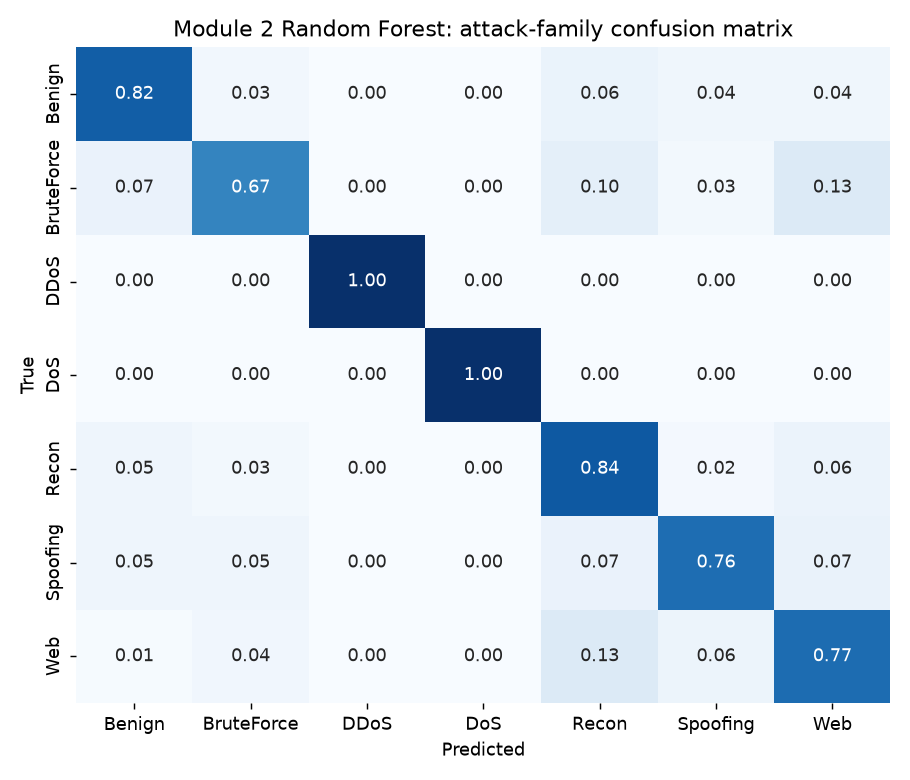
\includegraphics[width=0.65\textwidth]{m2_family_confusion.png}
\caption{Normalised attack-family confusion matrix of the Random Forest on the test records.}
\label{fig:m2family}
\end{figure}

\begin{figure}[htbp]
\centering
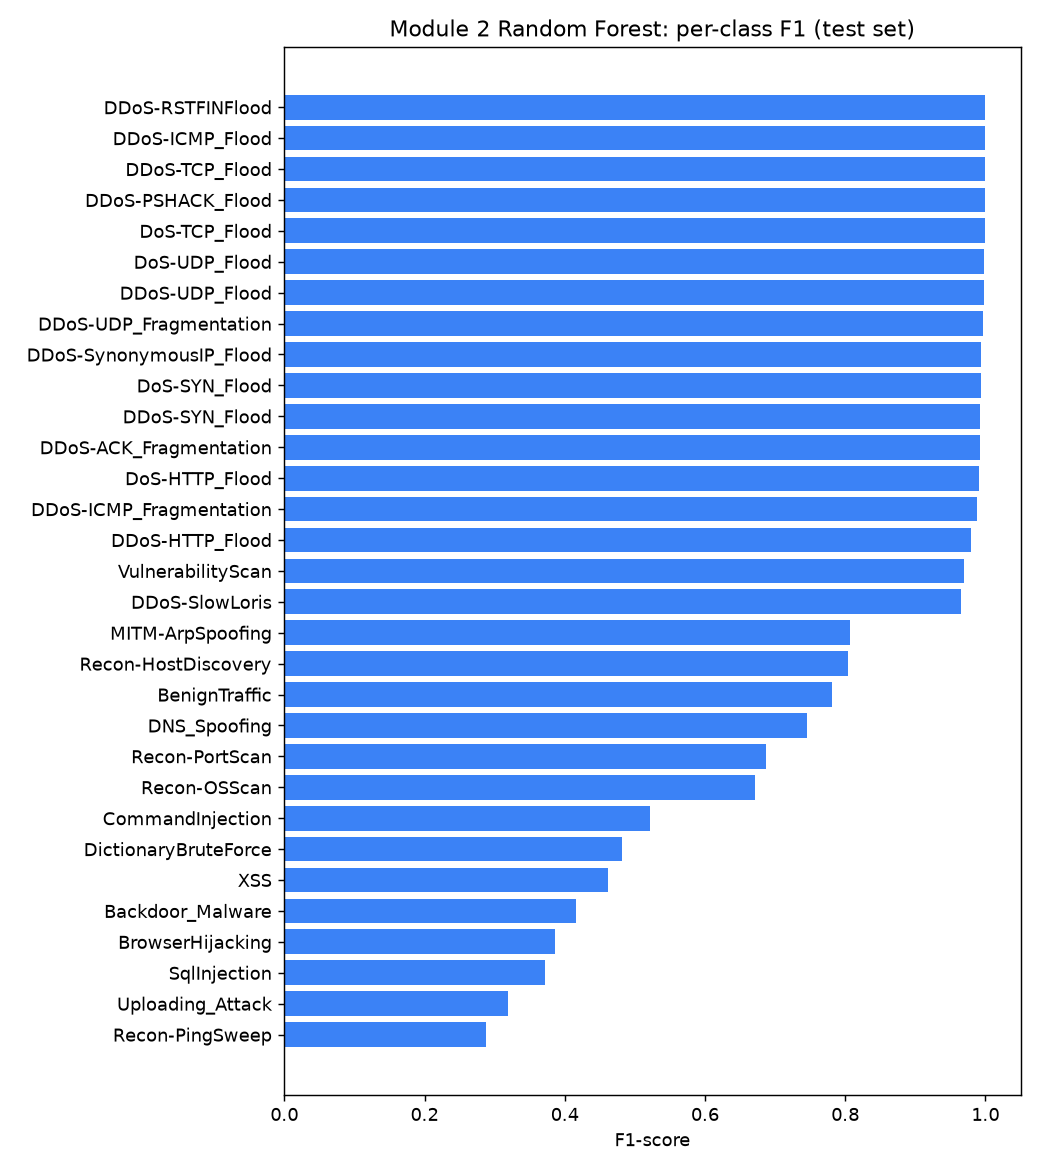
\includegraphics[width=0.7\textwidth]{m2_per_class_f1.png}
\caption{Per-class F1-score of the Random Forest on the test records.}
\label{fig:m2perclass}
\end{figure}

\subsection{Computational Efficiency}
The efficiency of the proposed system is measured using model size, inference time and the share of windows that need the second module. The INT8 model needs 16.2~KB, which is 74.6\% smaller than its FP32 version (63.6~KB), and it classifies a window of 20 records in a median of 0.55~ms, compared with 6.29~ms for the Random Forest. The Random Forest is the more accurate classifier, but at 118.3~MB it is better suited to a gateway than to a constrained device, where the INT8 model is the intended choice. Both latencies are measured with the same Python runtime on the same CPU, so the difference comes from the models themselves. In the proposed system, the first module checks the traffic and sends only suspicious traffic to the second module (Fig.~\ref{fig:routing}). In the end-to-end stream of 390 windows, the first module classified 214 windows (54.9\%) as normal, and these windows bypassed the second and third modules entirely, while 46 suspicious and 130 attack windows (45.1\%) were sent for further analysis. The stream deliberately contains a large share of attack windows (41\%); in operational IoT networks, where most of the traffic is normal, the share of windows that skip the classifier would be even higher.

\begin{figure}[htbp]
\centering
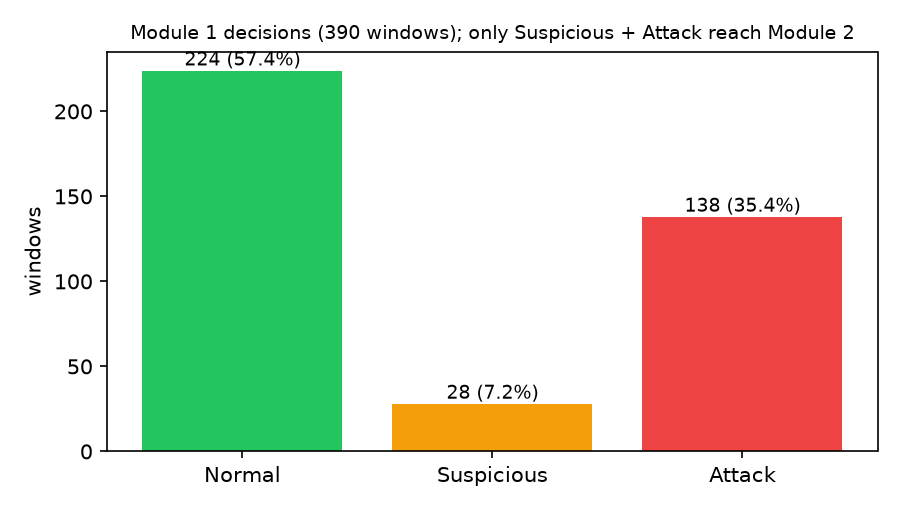
\includegraphics[width=0.75\textwidth]{fig_module2_invocation.png}
\caption{Distribution of the 390 end-to-end windows by the fuzzy logic decision; only suspicious and attack windows are sent to Module 2.}
\label{fig:routing}
\end{figure}

\subsection{Parameter Sensitivity}
The two main parameters of the first module are the window size $W$ and the sensitivity parameter $k$ of the adaptive MAD baseline, so both of them are varied to see how the results change (Fig.~\ref{fig:sensitivity}). For the window size, the F1-score of the final fuzzy logic was 99.19\% at $W=10$, 99.80\% at $W=20$ and 100\% at $W=50$ and $W=100$, evaluated on 15 windows per class for each size. A very small window contains too few records to estimate the variation of the IAT, while a larger window is slightly more accurate but needs more records before a decision can be taken, so it reacts more slowly to an attack and mixes the attack traffic with normal traffic when an attack starts or ends inside the window; therefore $W = 20$ is used as a balance. For the adaptive MAD baseline, increasing $k$ from 2.0 to 4.0 reduced the alarm rate from 3.90\% to 0.44\%, which shows that this method can only trade one type of error against the other and cannot separate the attack windows from the normal ones; $k = 3.0$ is used in all the reported results.

\begin{figure}[htbp]
\centering
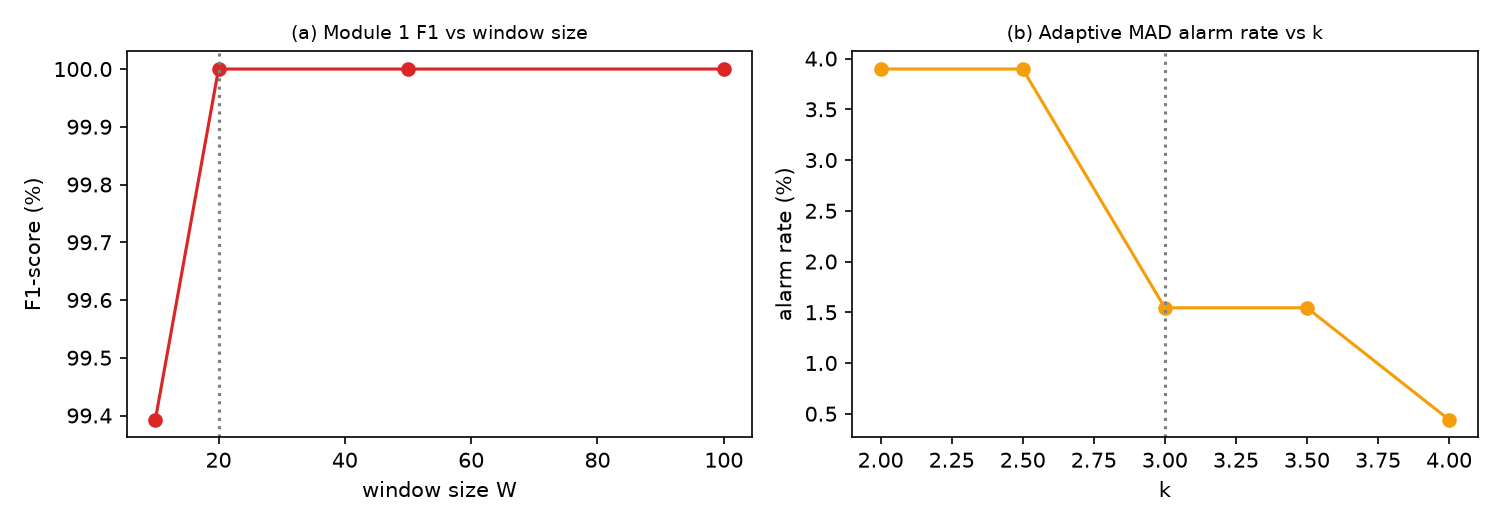
\includegraphics[width=\textwidth]{fig_parameter_sensitivity.png}
\caption{(a) Effect of the window size $W$ on the F1-score of the final fuzzy logic. (b) Effect of the sensitivity parameter $k$ on the alarm rate of the adaptive MAD baseline. The dotted lines mark the values used in this work, $W=20$ and $k=3.0$.}
\label{fig:sensitivity}
\end{figure}

\subsection{Held-Out Attack Analysis}
The system is tested using the three held-out Mirai attack categories, Mirai-greeth\_flood, Mirai-greip\_flood and Mirai-udpplain, which are not included in the classifier's training classes, in order to test how well the system handles unseen attacks (Fig.~\ref{fig:zeroday}). The final fuzzy logic detected 100\% of the held-out attack windows, because it only compares the traffic with normal behaviour and does not depend on attack labels, whereas the timing-only fuzzy logic detected 33.33\% and the static CV and adaptive MAD methods detected none. The open-set check of the second module labelled 100\% of the Mirai windows as unknown, while only 4.44\% of the windows of known attacks were wrongly labelled as unknown. The median zero-day score was 3.69 for the Mirai windows and 0.52 for the known attack windows, against a threshold of 1. In our earlier experiments, the confidence-based rejection of the classifier detected 0\% of the Mirai windows, and the unseen floods were classified as known attacks such as DDoS-UDP\_Fragmentation and DoS-UDP\_Flood. Measuring the distance to the known traffic, instead of relying on the confidence of the classifier, prevents the system from forcing unseen attacks into a known class.

\begin{figure}[htbp]
\centering
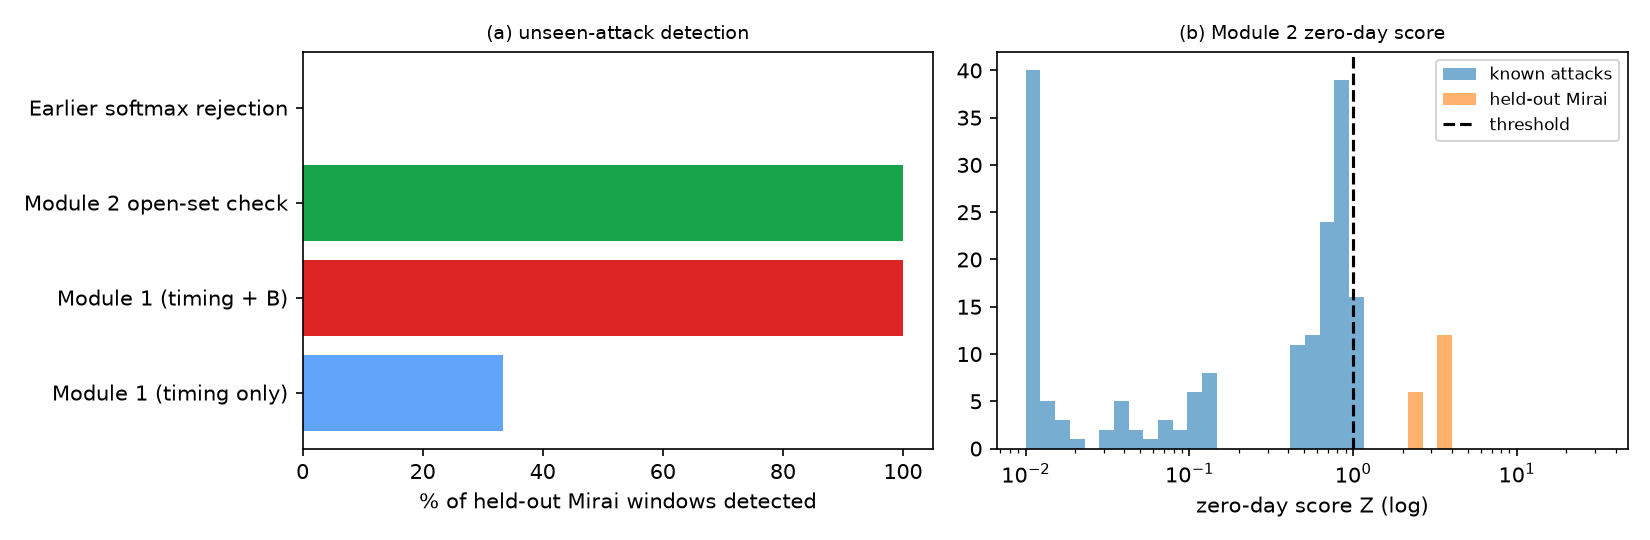
\includegraphics[width=\textwidth]{fig_zero_day_analysis.png}
\caption{Held-out Mirai analysis. (a) Share of the unseen attack windows detected by each stage, including the confidence-based rejection of our earlier classifier. (b) Distribution of the zero-day score $Z_t$ of the second module for known attack windows and held-out Mirai windows, with the threshold at 1.}
\label{fig:zeroday}
\end{figure}

\subsection{Mitigation Performance}
The mitigation module is evaluated through the full pipeline, driven by the predictions of the second module, on 645 windows covering all 33 attack classes and normal traffic. 491 windows reached the third module: 86.56\% of them through a class policy and 13.44\% through the zero-day route. The known attacks were routed to the policy family of their true class in 94.39\% of the cases, and 95.72\% of the plans were verified by the first module to bring the attack risk below 0.35. The mean risk fell from 0.73 to 0.17, and the mean CV of the windows after mitigation was 0.99, which is close to the normal value of 1.0. 85.1\% of the plans needed only a single action, and the first action removed 82.31\% of the packet volume of the targeted records on average. Blocking or isolation was needed in 32.79\% of the plans, and 62.12\% of the plans could start automatically.

Table~\ref{tab:m3family} and Fig.~\ref{fig:m3family} show the results for each policy family. The filtering families (volumetric flood, TCP state exhaustion, fragmentation and slow application) start automatically and are resolved in 94--100\% of the windows. The reconnaissance, spoofing, web, credential and malware plans need an analyst, because their first action blocks traffic or the confidence of the second module on these classes is below the policy threshold. The botnet policy was not used, because its only CICIoT2023 classes are the held-out Mirai classes. The distribution of the first actions is given in Table~\ref{tab:actions}.

\begin{table}[htbp]
\tbl{Module 3 results per policy family (645-window evaluation driven by Module 2 predictions).}
{\small
\begin{tabular}{lccccc}
\toprule
Policy family & Windows & Resolved & Automatic & Single stage & Volume removed \\
\midrule
Volumetric flood        & 90 & 94.4\%  & 100\% & 74.4\%  & 77.0\% \\
TCP state exhaustion    & 60 & 95.0\%  & 100\% & 70.0\%  & 76.0\% \\
Fragmentation           & 45 & 100\%   & 100\% & 88.9\%  & 83.3\% \\
Slow application        & 45 & 100\%   & 100\% & 93.3\%  & 76.5\% \\
Reconnaissance          & 60 & 96.7\%  & 0\%   & 96.7\%  & 97.1\% \\
Spoofing / MITM         & 32 & 96.9\%  & 0\%   & 96.9\%  & 93.8\% \\
Web application         & 66 & 90.9\%  & 0\%   & 84.8\%  & 84.3\% \\
Credential              & 12 & 100\%   & 0\%   & 100\%   & 90.3\% \\
Malware / backdoor      & 15 & 86.7\%  & 0\%   & 100\%   & 100\% \\
Zero-day (traffic shape)& 66 & 97.0\%  & 98.5\% & 83.3\% & 72.1\% \\
\midrule
All                     & 491 & 95.7\% & 62.1\% & 85.1\% & 82.3\% \\
\bottomrule
\end{tabular}}
\label{tab:m3family}
\end{table}

\begin{figure}[htbp]
\centering
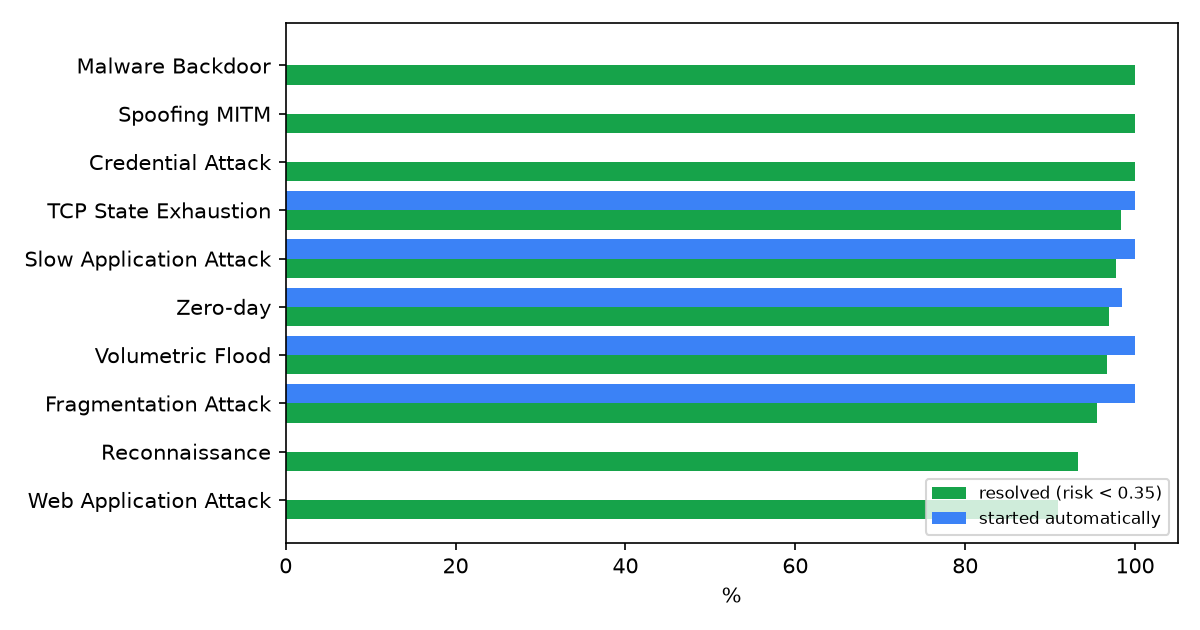
\includegraphics[width=0.8\textwidth]{fig_mitigation_by_family.png}
\caption{Share of windows resolved (risk below 0.35 after mitigation) and share of plans started automatically, for each policy family.}
\label{fig:m3family}
\end{figure}

\begin{table}[htbp]
\tbl{First mitigation actions selected over the 645-window evaluation.}
{\begin{tabular}{llc}
\toprule
Action & Action class & Windows \\
\midrule
RATE\_LIMIT\_SOURCE            & FILTER & 155 \\
ACTIVATE\_WAF\_RULE            & FILTER & 66 \\
BLOCK\_SCANNING\_SOURCE        & BLOCK  & 61 \\
ENABLE\_SYN\_COOKIES           & FILTER & 60 \\
DROP\_MALFORMED\_FRAGMENTS     & FILTER & 45 \\
LIMIT\_CONCURRENT\_CONNECTIONS & FILTER & 45 \\
ENFORCE\_ARP\_DNS\_INTEGRITY   & BLOCK  & 32 \\
QUARANTINE\_ENDPOINT           & BLOCK  & 15 \\
THROTTLE\_AUTH\_ATTEMPTS       & FILTER & 12 \\
\midrule
Total windows sent to Module 3 & & 491 \\
\bottomrule
\end{tabular}}
\label{tab:actions}
\end{table}

For the held-out Mirai attacks, all 45 windows reached the third module and took the zero-day route. 37 of them (82.2\%) were identified as constant-rate floods from their traffic shape alone, without knowing the name of the attack. The other 8 were unclassified anomalies, usually because a benign record that the second module had marked as attack broke the regular timing. 97.78\% of the Mirai windows were resolved. The 66 zero-day plans also include known-attack windows that the second module marked as unknown, which were contained by the same shape-based ladders. This shows that even when the classifier cannot name an attack, the system can still take a suitable containment action using the behaviour measured by the first module.

\subsection{End-to-End Performance}
In the end-to-end stream of 390 windows (160 attack windows and 230 normal windows), the first module detected 158 of the 160 attack windows (98.75\%) and raised 18 false alarms on the 230 normal windows (7.8\%). 54.87\% of the windows bypassed the second and third modules. The second module cleared 13 of the 18 false alarms as benign, so only 5 normal windows reached the third module, and since their ladders include blocking, they would wait for an analyst's approval in deployment. The third module executed 163 plans, 74.85\% through a class policy and 25.15\% through the zero-day route, and 159 of them (97.55\%) were verified to bring the risk below 0.35: 143 with the first action and 16 after escalating to the second. The mean risk fell from 0.78 to 0.16, and 74.23\% of the plans could start automatically.

\subsection{Limitations}
The CICIoT2023 CSV files do not contain the raw packet timestamps, so the timing analysis relies on the IAT feature provided by the dataset, and since the CSV rows are shuffled, the evaluation windows are assembled from the test records rather than taken from a continuous capture. The network controller of the third module is simulated, and the efficacy values of the actions are assumptions rather than measurements. The rare web and reconnaissance classes have few records, which limits their per-class F1-score. The false-positive rate of the first module is estimated from a small number of normal windows (40 in the detector comparison and 230 in the end-to-end stream), and the Random Forest model is large (118.3~MB). Finally, the latency was measured on a desktop CPU, and measurements on physical IoT hardware are left for future work.


% =====================================================================================
\section{Conclusion}
% =====================================================================================
This study addressed the problem of detecting, classifying and mitigating attacks in resource-constrained IoT networks, where IoT devices can't run a heavy model on every traffic window and unseen attacks are difficult to identify. Our proposed system uses the inter-arrival time of the traffic in sliding windows, and a Mamdani fuzzy inference system combines the coefficient of variation, packet rate and IAT deviation with a behaviour deviation learned only from normal traffic to find the attack risk of every window. On the CICIoT2023 dataset, the fuzzy logic achieved 99.77\% recall and a 99.81\% F1-score with a 5.0\% false-positive rate, whereas the static CV and adaptive MAD methods detected only 4.39\% and 1.44\% of the attack windows and the timing features alone detected 15.91\%, and it detected 100\% of the unseen Mirai windows. Only the suspicious or attack windows are forwarded to the classifiers, due to which 54.9\% of the windows of the end-to-end stream bypassed the second module. The Random Forest identified 31 known classes with 90.85\% accuracy (93.42\% at family level and 94.56\% at window level), the INT8 quantized neural network is 74.6\% smaller than its FP32 version with 98.5\% prediction agreement and runs in 0.55~ms per window, and the nearest-neighbour open-set check labelled all unseen Mirai windows as unknown. Finally, the mitigation module routed 94.4\% of the known attacks to the correct one of 10 policy families, contained the unseen attacks through ladders chosen from their traffic shape, and verified 95.7\% of the mitigations across all 33 attack classes by re-running the fuzzy logic. Future work will evaluate the system on raw packet captures with real timestamps, deploy the INT8 model and the mitigation actions on physical IoT gateways, and improve the classification of the rare web and reconnaissance attacks.

\section*{Disclosure statement}
The authors report there are no competing interests to declare.

\section*{Data availability statement}
The CICIoT2023 dataset used in this study is publicly available from the Canadian Institute for Cybersecurity. The implementation of the proposed system is available at \url{https://github.com/sahamon-141/Capstone-2}.

\bibliographystyle{tfp}
\bibliography{interacttfpsample}

\end{document}
